% Use the option review to obtain double line spacing
\documentclass[review,3p]{elsarticle}

%% Use the options 1p,twocolumn; 3p; 3p,twocolumn; 5p; or 5p,twocolumn
%% for a journal layout:
%% \documentclass[final,1p,times]{elsarticle}
%% \documentclass[final,1p,times,twocolumn]{elsarticle}
%% \documentclass[final,3p,times]{elsarticle}
%% \documentclass[final,3p,times,twocolumn]{elsarticle}
%% \documentclass[final,5p,times]{elsarticle}
%% \documentclass[final,5p,times,twocolumn]{elsarticle}
%%%%%%%%%%%%%%%%%%%%%%%%%%%%%%%%%%%%%%%%%%%%%%%%%%%%%%%%%%%%%%%%%%%%%
%% Place any additional packages needed here.  Only include packages
%% which are essential, to avoid problems later.
%%%%%%%%%%%%%%%%%%%%%%%%%%%%%%%%%%%%%%%%%%%%%%%%%%%%%%%%%%%%%%%%%%%%%
\usepackage{mciteplus}
\usepackage{natbib}
\usepackage{tabularx}
\usepackage{booktabs,multirow,longtable,multirow,subfigure,graphicx,epstopdf}
\usepackage{amsmath,amsfonts,amssymb,nicefrac}
\usepackage[english]{babel}
\usepackage{geometry}
\usepackage{color}
\usepackage{hyperref}
\biboptions{comma,round}
\journal{Journal of Process Control}

%%%%%%%%%%%%%%%%%%%%%%%%%%%%%%%%%%%%%%%%%%%%%%%%%%%%%%%%%%%%%%%%%%%%%
%% If issues arise when submitting your manuscript, you may want to
%% un-comment the next line.  This provides information on the
%% version of every file you have used.
%%%%%%%%%%%%%%%%%%%%%%%%%%%%%%%%%%%%%%%%%%%%%%%%%%%%%%%%%%%%%%%%%%%%%
%\listfiles

%%%%%%%%%%%%%%%%%%%%%%%%%%%%%%%%%%%%%%%%%%%%%%%%%%%%%%%%%%%%%%%%%%%%
%% Place any additional macros here.  Please use \newcommand* where
%% possible, and avoid layout changing macros (which are not used
%% when typesetting).
%%%%%%%%%%%%%%%%%%%%%%%%%%%%%%%%%%%%%%%%%%%%%%%%%%%%%%%%%%%%%%%%%%%%%
\newcommand*{\mycommand}[1]{\texttt{\emph{#1}}}
\renewcommand\[{\begin{equation}}
\renewcommand\]{\end{equation}}

\definecolor{gray}{rgb}{0.5,0.5,0.5}
\usepackage[]{changes}

%%%%%%%%%%%%%%%%%%%%%%%%%%%%%%%%%%%%%%%%%%%%%%%%%%%%%%%%%%%%%%%%%%%%%
%% Meta-data block
%% ---------------
%% Each author should be given as a separate \author command.
%%
%% Corresponding authors should have an e-mail given after the author
%% name as an \email command.
%%
%% The affiliation of authors is given after the authors; each
%% \affiliation command applies to all preceding authors not already
%% assigned an affiliation.
%%
%% The affiliation takes an option argument for the short name.  This
%% will typically be something like "University of Somewhere".
%%
%% The \altaffiliation macro should be used for new address, etc.
%%%%%%%%%%%%%%%%%%%%%%%%%%%%%%%%%%%%%%%%%%%%%%%%%%%%%%%%%%%%%%%%%%%%%
\begin{document}
\begin{frontmatter}
\title{Data-driven adaptive multiple model system utilizing growing self-organizing maps}
%% use optional labels to link authors explicitly to addresses:
%% \author[label1,label2]{<author name>}
%% \address[label1]{<address>}
%% \address[label2]{<address>}

\author[dow]{Bo Lu \corref{cor1}}
\ead{blu2@dow.com}
\author[vsli]{John Stuber}
\author[uta]{Thomas F. Edgar}
\cortext[cor1]{Corresponding author}
\address[dow]{Analytical Technology Center, The Dow Chemical Company, Freeport, Texas}
\address[vsli]{Smart Manufacturing Systems Group, VLSIP Technologies Inc., Richardson, TX}
\address[uta]{McKetta Department of Chemical Engineering, The University of Texas at Austin, Austin, Texas}
%%%%%%%%%%%%%%%%%%%%%%%%%%%%%%%%%%%%%%%%%%%%%%%%%%%%%%%%%%%%%%%%%%%%%
%% The document title should be given as usual
%% A short title can be given as a *suggestion* for running headers.
%%%%%%%%%%%%%%%%%%%%%%%%%%%%%%%%%%%%%%%%%%%%%%%%%%%%%%%%%%%%%%%%%%%%%


%%%%%%%%%%%%%%%%%%%%%%%%%%%%%%%%%%%%%%%%%%%%%%%%%%%%%%%%%%%%%%%%%%%%%
%% The manuscript does not need to include \maketitle, which is
%% executed automatically.  The document should begin with an
%% abstract, if appropriate.  If one is given and should not be, the
%% contents will be gobbled.
%%%%%%%%%%%%%%%%%%%%%%%%%%%%%%%%%%%%%%%%%%%%%%%%%%%%%%%%%%%%%%%%%%%%%
\begin{abstract}
Data-driven soft sensors have seen tremendous development and adoption in both academia and industry. However, one of the challenges remaining is modeling process drifts, degradation and discontinuities in steady-state. Since processes are never truly operating at a steady-state, it is often difficult to assess how much and what types of process data are needed for training and model maintenance in the future. A purely adaptive model maintenance strategy struggles against discontinuities such as preventive maintenance or catalyst changes. In mixture modeling and multi-model systems, the overall modeling structure is fixed and only local coefficients are adapted. In addition, multiple model systems require large amount of training data to initialize. In this paper, we propose an adaptive multiple model system utilizing growing self organizing map to model processes with drifts and discontinuities. Simple model update mechanisms such as recursive model update or moving window model update is not sufficient to deal with discontinuities such as abrupt process changes or grade transitions. For these scenarios, our approach combines projection based local models (Partial Least Squares) with growing self-organizing maps to allow for flexible adjustments to model complexity during training, and also later in online adaptation. This flexible framework can also be used to explore new datasets and rapidly develop model prototypes. We demonstrate the effectiveness of our proposed method through a simulated test cases and an industrial case study in predicting etch rate of a plasma etch reactor.
\end{abstract}

\begin{keyword}
multiple model systems \sep  adaptive model \sep  growing self-organizing map \sep  growing structure multiple model systems \sep  soft sensor \sep  data-driven modeling \sep  PLS \sep  PCA \sep  projection to latent structure \sep  partial least squares
\end{keyword}
\end{frontmatter}
\index{GSMMS}%
\index{GSMMS!Growing structure multiple model systems}%
\label{sec:gsmms}
\section{Introduction}
Industrial manufacturing systems are becoming increasingly complex and
sophisticated due to more stringent requirements on efficiency, product quality and asset utilization. The additional system complexity is possible due to advancements in control, real-time optimization and continuous process
improvement. As a result of these complex integrated systems, it becomes increasingly challenging to deal with monitoring and prediction of key quality parameters. Considerable work have gone into improving modern soft sensors performance by increasing their robustness against missing data or poor data \cite{Guo2014,Zhu2015,Godoy2017}, improved handling of system dynamics \cite{Shang2015}, and improved model updating \cite{Chen2017,Cao2014}. Yet, many of these systems operate in multiple production modes which can be characterized by throughput, load, level, recipe and product grades \cite{Qin2012}.
Traditional methods such as static soft sensor models are ill-suited for
these complex systems. Multivariate data-driven models using Principal Component Analysis (PCA) and Partial Least Squares (PLS) also face challenges due to inherent nonlinearity, process drifts, multiple operating modes and complex fault signatures
\cite{Kadlec2011}. 

Since the data generated from these systems naturally have multi-modal
distributions \cite{Yu2008}, a ``divide and conquer'' approach is commonly
taken to partition the data into sub-regions that can be approximated using
simple local models. After satisfactory performance is achieved at the local
level, selection of the current operating mode at a supervisory layer can then be used to smooth local model
results for better prediction of the overall system. Liu proposed a method to detect changes in operating mode to select the best predictor in a multi-modal soft sensor application in \cite{Liu2016}. Dunia and Edgar
formulated a multi-state PLS framework where transitions between states are
smoothed using a k-means clustering smoothing mechanism \cite{Dunia2012}.
Kadlec et al. proposed an incremental learning adaptive soft sensor system
that generates operating modes based on prediction residual performance and
combines the local model predictions using a Bayesian-inference based
validity function approach \cite{Kadlec2011a}. There are also many other
published works in this area\cite{Liu2007,Liu2009,Lin2007,Eriksson2009}.
Common challenges associated with these approaches are:
\begin{enumerate}
\item Partitioning of the operating space needs to be determined before
    local model training \cite{Kadlec2011a, Dunia2012}.
\item Operating modes that have limited training data can lead to
    numerical instability \cite{Kadlec2011a, Eriksson2009}.
\item Local model and supervisory structural layer are often trained separately \cite{Dunia2012}.
\item It is often difficult to implement these complex models online in an industrial environment.
\end{enumerate}

On the other hand, mixture models and kernel density
estimates based methods directly assumes that the underlying data distribution is
non-Gaussian and multi-modal \emph{without any easily identifiable class
labels}. In these methods, mixture models do not
require apriori definition of a multi-model structure. Yu and Qin
\cite{Yu2008} proposed using finite Gaussian Mixtures to monitor industrial process data. They
obtained results superior to conventional multivariate monitoring schemes
on the Tennessee-Eastman plant simulation. Thissen et al. applied finite Gaussian
mixture models to industrial data of a fiber spinning process and found much
higher sensitivity to faults using Gaussian Mixture Models
\cite{Thissen2005}. \added{Sammaknejad et al. modeled the transition among operating states as a Hidden Markov process where the transition probabilities are adapted online. Their approach was applied in montioring an oil sand froth treatment process \cite{Sammaknejad2015}.} Some of the other works using mixtures of distributions are
\cite{Yu2011,yoo2007multi,zhao2010statistical,zhao2004monitoring}. \added{Through reviewing these works, we can observe that this class of methods face the following challenges}:
\begin{enumerate}
\item difficult to troubleshoot due to the lack of transparency
\item difficult to implement online due to heavier computational
    requirements
\item stability of online adaptation of these Gaussian mixtures has not
    been thoroughly studied.
\end{enumerate}
Batch process data from semiconductor manufacturing are particularly
challenging to model due to the following characteristics:
\begin{itemize}
    \item \textbf{high-mix manufacturing}, upstream and downstream
        processes could change depending on product and production thread.
        Therefore, unmeasured disturbances could affect process modeling
        results.
    \item \textbf{large number of measurements}, high dimensional data
        resulting from unfolding of batch trajectories
    \item \textbf{threaded production}, multiple recipes are ran on the
        same tool. As a result, some un-popular recipes might have little
        data available for model building.
    \item \textbf{nonlinearity}, input-output relationships are not linear
    \item \textbf{process degradation}, input-output relationships drift
        overtime
\end{itemize}
To improve upon existing works, our proposed new approach attempt to satisfy the following:
\begin{itemize}
  \item Does not rely on class label information
  \item Does not require large amount of training data to initialize
  \item Can be easily extended for online adaptation
  \item Produces interpretable local models and diagnostics for troubleshooting
\end{itemize}
To this end, the work of growing structure multiple model systems proposed by
Liu et al. \cite{Liu2009} and Bleakie et al. \cite{Bleakie2013} inspired the
development of a hybrid multiple model system that combines PLS local models with a Growing self-organizing Map to form an integrated framework suitable for batch data from semiconductor
manufacturing.

\section{Growing self-organizing Map}
Growing self-organizing map (GSOM) is a subclass of self-organizing maps (SOM),
which is a type of unsupervised machine learning technique. SOM is also a special case of an artificial neural network. Its primary purpose is to map high dimensional data
onto a lower-dimensional space. It is also called a Kohonen map \cite{Kohonen1982}. 
Different from clustering algorithms and other artificial neural networks, SOMs attempt to preserve the topology of the input space by modeling the connections between clusters. As a
result, these topological information can be used to improve prediction, training, and model
update. 
GSOM makes no prior assumption about the
size of the map and allows the algorithm to learn the model parameters at
run-time. 
An example of the topology in a GSOM is given in Figure~\ref{fig:gsom_example}, where GSOM is able to preserve the spiral geometry in the reduced dimensional space.
\begin{figure}.
  \centering
  \includegraphics[width=0.55\textwidth]{figures/gsmms/SOMvsPCA.png}\\
  \caption{Example of SOM vs GSOM under different tuning parameters, figure taken from \cite{Akinduko:2016:SOM:2957613.2957681}}\label{fig:gsom_example}
\end{figure}

Just like other artificial neural networks; GSOM requires training before it
becomes useful. The classic GSOM undergoes three stages of training:
\begin{description}
  \item[initialization] where small number of nodes and the topological
      structure parameters are initialized.
  \item[growing] where training input is presented to GSOM to successively
      minimize the vector quantization error of the input data. Existing
      nodes will be relocated to new positions, and new nodes will be added
      as the algorithm sees fit.
  \item[fine-tuning] final adjustment of node positions according to
      training data.
\end{description}

In the proposed approach, since the structural learning phase (training the
GSOM) is integrated with the local learning phase (training local PLS models), both training phases will be discussed together. First, the basic mathematical description of GSOM is introduced.

Given input and output data $\mathbf X (N \times P)$ and ${\mathbf y} (N \times 1)$, we can
define a feature vector for each observation
\[\mathbf{s}_i = [s_1\;s_2\;s_3\;s_4\ldots s_K]_i = [P(\mathbf{x}_i,\mathbf{x}_{i-1},\ldots),
Q(\mathbf{y}_i,\mathbf{y}_{i-1},\ldots)] \] where $P(\cdot)$ and $Q(\cdot)$
are features selection functions. These functions can either reduce feature
space dimension by projecting $X$ onto a lower dimensional space \added{using techniques such as Principal Component Analysis (PCA) or Independent Component Analysis (ICA)}, expand
feature space by introducing nonlinear terms or lagged variables. \added{Determining the appropriate feature selection function will depend on the dataset being modeled and also the prior knowledge of the process.} \deleted{In
practice, using only $X$ variables with no transformation is a good starting
point for exploratory analysis.}

Once the feature vectors are defined, SOM is then trained on the features. A trained SOM has the location of its nodes and the neighborhood connections fully specified. This can be represented graphically in Figure~\ref{fig:gsmms_parameters}. Each node contain a codebook vector and a local model. The codebook vector is a coordinate of the node and has the same dimension as the feature space:
\[
\xi_m := [s_1\;s_2\;s_3\;s_4\ldots s_K]
\]
where $m$ is the node index and $K$ is the dimension of the feature space. The total number of nodes $M$ is determined during training.

\replaced{Given a fully parameterized SOM}{To partition the feature space into sub-regions}, the feature space can be partitioned into $M$ subspaces ($V_1, V_2, \ldots V_m$) each belonging to a node $m$ based on a distance metric:
\[{V_m} = \left\{ {{\bf{s}}:\left\| {{\bf{s}} - {{\bf{\xi }}_m}} \right\| \le \left\| {{\bf{s}} - {\xi _i}} \right\|,\forall i \in \left( {1,M} \right),i \ne m} \right\}\]

The quantization error of input $\mathbf s$ with respect to node $m$ is defined as:
\[
e(\mathbf s,\xi_m) = \left\| {{\bf{s}} - {\xi _m}} \right\|
\label{eqn:quantization_err}
\]

To find the best matching unit (BMU) $m$ given an feature vector $\mathbf s$, we compare the vector
quantization error of $\mathbf s$ with all possible SOM nodes $\xi_m, m = 1,2 \ldots M$ and look for the node with the smallest error:
\begin{equation}
BMU\left( {\bf{s}} \right) = \mathop {{\rm{argmin}}}\limits_m
\left\| {{\bf{s}} - {\xi _m}} \right\|,m = 1,2, \ldots M
\label{eqn:bmu}
\end{equation}

\added{Note that any given input feature $\mathbf s$ will always be assigned to a BMU even if the BMU assigned contain a large quantization error. The minimization of total quantization error occurs in the later training stage of the SOM.} The topological relationship of the SOM is stored in a symmetric binary
matrix, called the adjacency matrix $\mathbb A \;(M \times M)$, where M is
the number of nodes in the SOM. A node $i$ is said to be connected to node
$j$ if $\mathbb A(i,j) = 1$ (in this case, $\mathbb A(j,i)$ also equal to
$1$). The adjacency matrix can be visualized as connections between nodes on
a SOM. Figure~\ref{fig:gsmms_parameters} illustrates the adjacency matrix
visually using an example with 10 nodes. Each node is numbered with an index.
With respect to node 1, nodes 2,3 are its primary neighbors (immediately
adjacent) while nodes 4,5 are its secondary neighbors (separated by one node
in between).
\begin{figure}.
  \centering
  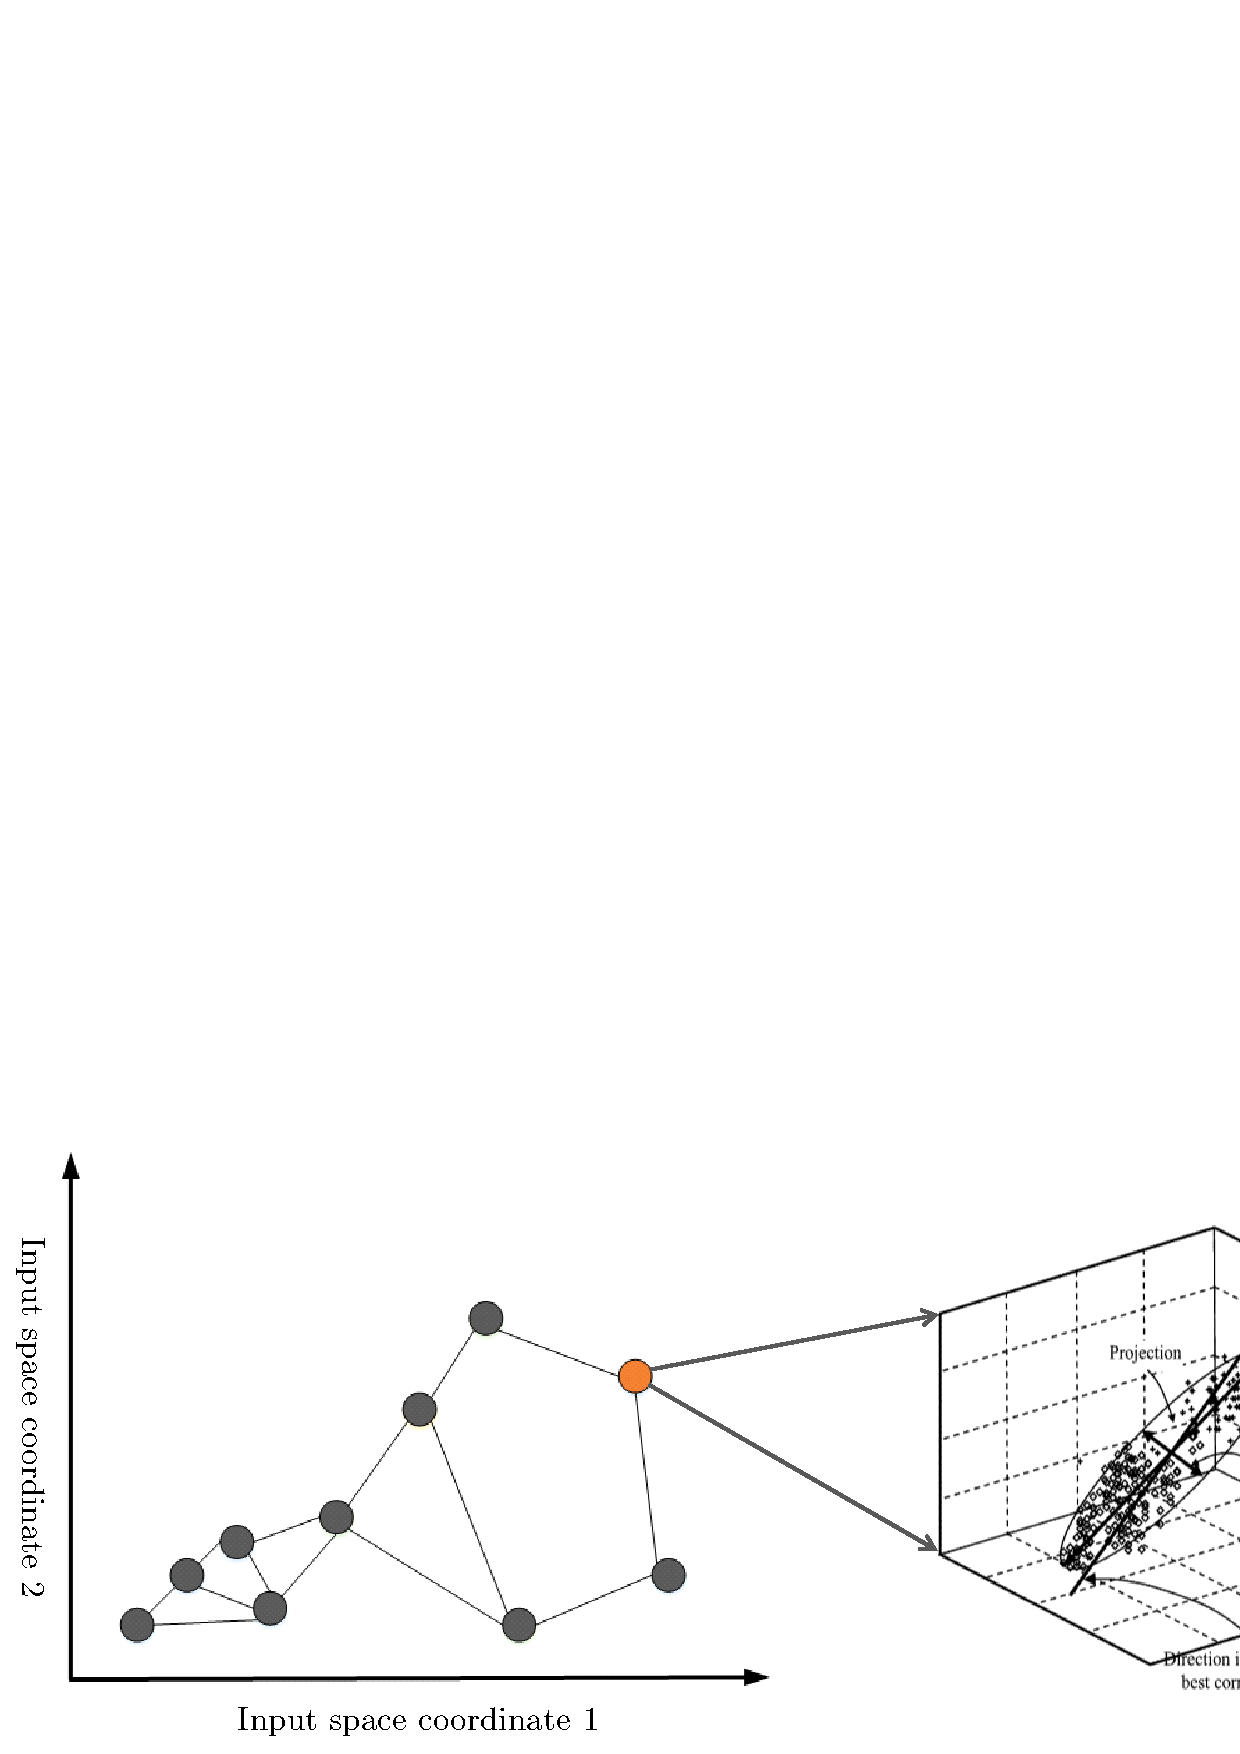
\includegraphics[width=0.95\textwidth]{figures/gsmms/gsmms_parameters.png}\\
  \caption{Parameters that need to be specified in a MMS system: The GSOM network, and local model at each node, which constitutes a growing structure MMS (GSMMS)}\label{fig:gsmms_parameters}
\end{figure}


\section{Growing Structure Multiple Model Systems}
 Growing Structure Multiple Model Systems (GSMMS) are composed of a GSOM network and all the local models at each node. Most of multiple modeling techniques divide the training of the model into two phases: supervisory layer learning and local model
learning as shown in Figure~\ref{fig:other_methods_flowchart}. Although this approach is straightforward and simple to implement, there are some disadvantages. For instance, the number of local models is usually fixed and
cannot be changed easily. In addition, there is no feedback of local model performance to improve multi-modal assignment. However, in our proposed approach, the two training phases are integrated as shown in
Figure~\ref{fig:gsmms_training}. The overall algorithm initializes with a
small SOM and then iterate to adapt the SOM structure and the corresponding
local models. There are two iteration loops in the proposed training scheme. The outer loop incrementally add nodes until the global fitting error reaches a minimum (corresponding to the growing phase in GSOM training). The inner loop adjusts
the codebook of each node ($\xi_m$) to find the optimal coordinate location of codebook vectors.

\begin{figure}
  \centering
  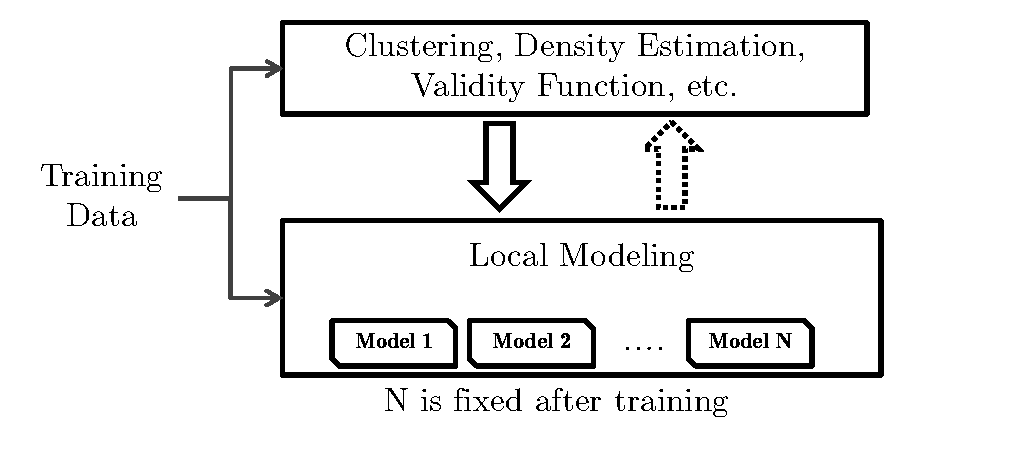
\includegraphics[width=0.95\textwidth]{figures/gsmms/other_methods_flowchart.eps}\\
  \caption{Basic flow of information in conventional multiple model systems}\label{fig:other_methods_flowchart}
\end{figure}
\begin{figure}.
  \centering
  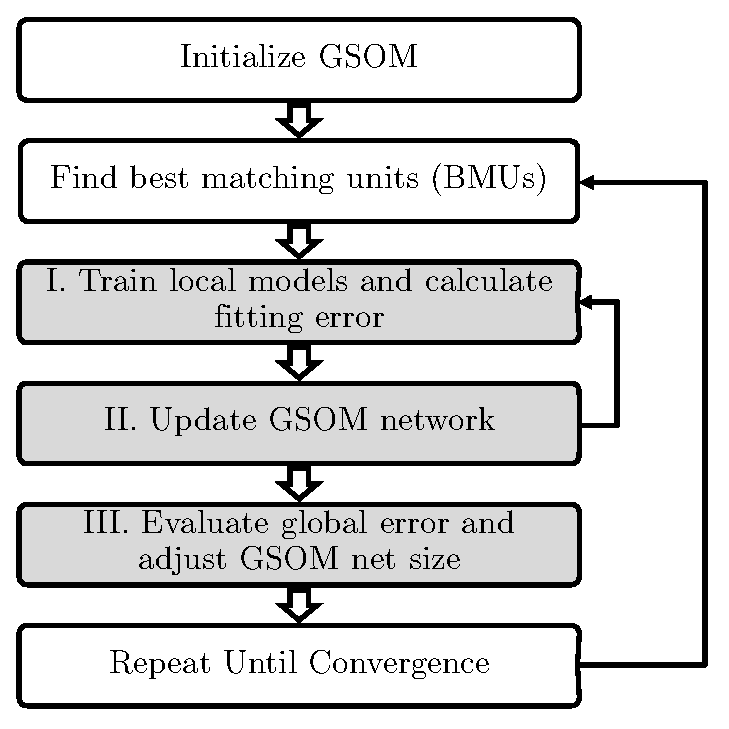
\includegraphics[width=0.6\textwidth]{figures/gsmms/gsmms_training.eps}\\
  \caption{Overall training procedure for GSMMS models}\label{fig:gsmms_training}
\end{figure}


\subsection{Initialization}
To initialize the GSOM for training, the initial codebooks vector ${\mathbf \xi_m}$ and the initial adjacency matrix $\mathbb A$ need to be specified. The initial codebook vector ${\mathbf \xi_m}$
is randomly sampled from the training features similar to k-means clustering initialization. Through trial and error, a network size of three nodes was found to be the optimal initial network size. The adjacency matrix $\mathbb A$ of the three node GSOM is defined as:
\[\mathbb{A} = \left[ {\begin{array}{*{20}{c}}
0&1&1\\
1&0&1\\
1&1&0
\end{array}} \right]\]
This initial $\mathbb A$ connects all three nodes with each other,
forming a triangle if visualized graphically.

The $\mathbf{BMU}$ vector for all training input is then calculated using
Equation~\ref{eqn:bmu}.
\[
\mathbf{BMU} = \{BMU_i, i \in (1,N_\mathrm{samples})\}
\]
An observation is said to belong to node $m$ if the $BMU$ of this observation
is $m$. 
As the SOM undergoes training, the membership association of each observation will change. A Gaussian weighting function
$\mathbf{w}_m(\mathbf{ BMU},\mathbb A)$ returns the
weight of each observation with respect to the specific node $m$:
\begin{equation}
{w_m}\left( {BM{U_i},\mathbb A} \right) = \exp \left( {\frac{{ - dis\left( {m,BM{U_i},\mathbb A} \right)}}{{2{\sigma ^2}}}} \right),m = 1,2,..M
\label{eqn:gsmms_weight}
\end{equation}
where $\sigma^2$ is a parameter that defines the effective range of the
weighting function, and $dis(m,BMU_i,\mathbb A)$ is the topological distance
given the current network configuration $\mathbb A$. \added{The topological distance is defined to take on integer values such as $1,2,3 \ldots M$ to simplify graph computation and improve stability.} It is best explained visually through Figure~\ref{fig:gsmms_topdis}. For nodes directly adjacent to $m$, the value is 1. For its secondary neighbors, the value is 2 and so on. 
This calculation can be carried out efficiently using Breath-first algorithms \cite{Russell2009}. \added{Note that nodes with the same topological distance might have different conventional geometric distances.}
\begin{figure}.
  \centering
  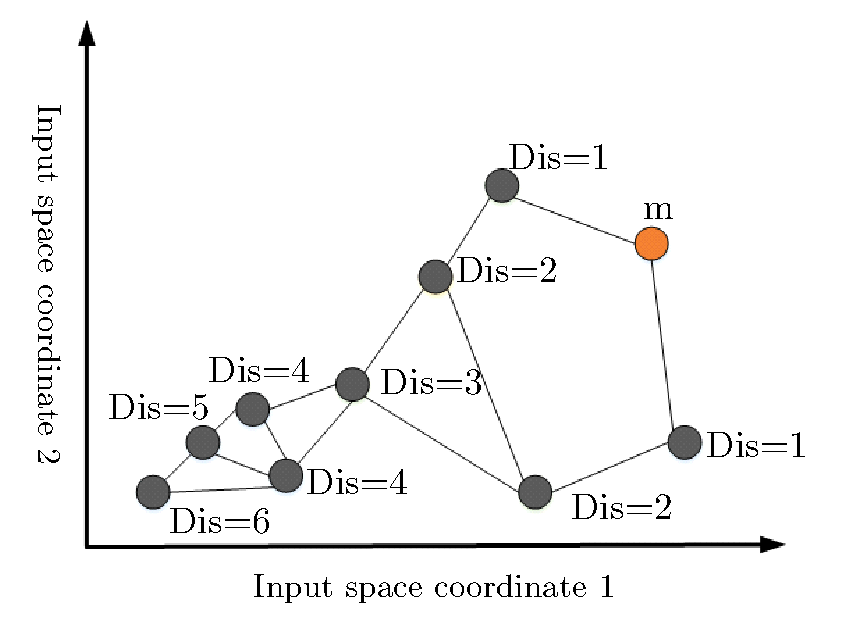
\includegraphics[width=0.8\textwidth]{figures/gsmms/gsmms_topdis.eps}\\
  \caption{Topological distance of each node with respect to node $m$}\label{fig:gsmms_topdis}
\end{figure}

The weighting function Equation~\ref{eqn:gsmms_weight} discounts data that are far away from the current node $m$ during training. 

\subsection{Sample weighted PLS local model fitting}
\added{To improve numerical stability and to allow smoother transitions between node boundaries, the local PLS models are trained using all input data; however, the data are sample weighted to discount the influence of input data outside of the current selected training node}. The sample weighted PLS can be written as:

\[\left[ {\mathbf{P},\mathbf{T},\mathbf{Q},\mathbf{U},\mathbf{W},\mathbf{\beta} } \right]_m = {\rm{weighted}}PLS\left( {\mathbf{X},\mathbf{y},\mathbf{w_m}} \right)\]
where $\mathbf{w_m} \in [0,1]$ \added{($N \times 1$)} is a vector of sample weights for node $m$:

\[
\mathbf{w_m} = \left[ w_m(BMU_1,\mathbb A), w_m(BMU_2,\mathbb A), \ldots, w_m(BMU_N,\mathbb A) \right]^T
\]

The sample weighted PCA algorithm accounts for different weights by applying the sample weights in the 
covariance matrix calculation.
The SIMPLS algorithm for PLS utilizes input-output covariance deflation to calculate
each successive PLS component vectors \cite{Jong1992}. The modified SIMPLS
algorithm shown in Table~\ref{tab:weighted_PLS} applies sample weights in the training input.
\begin{table}[htbp]
  \centering
  \caption{Algorithm details of sample weighted PLS algorithm}
  \begin{tabular}{cp{5in}}
    \toprule
    Step  & \\
    \midrule
    1 &  Construct weighting matrix $\Omega = diag(w_1,w_2,\ldots,w_P)$\\
    2 &  Mean center using weighted mean for $X, y$ matrices as follows:
$\begin{array}{l}
X_s = X - \bar X' ,{\bar X'} = {\left[ {1,1,...,1} \right]^T}\left[ {{{\bar x}_1},{{\bar x}_1}, \ldots ,{{\bar x}_M}} \right]\\
y_s = y - \bar y' \\
{{\bar x}_m} = \sum\limits_{n = 1}^N {{w_n}{x_{nm}}/\sum\limits_{n = 1}^N {{w_n}} }\\
\bar y' = \sum\limits_{n = 1}^N {{w_n}{y_n}} /\sum\limits_{n = 1}^N {{w_n}}\end{array}$\\
    3 &  Compute weighted cross product $\mathbf{ S = X_s^T\Omega {y_s}y_s^T\Omega {X_s}}$\\
      & Let $a = 1$\\
    4 & If $a = 1$, calculate $\mathbf{[r,s,c]} = SVD(\mathbf S)$ \\
      & If $a > 1$, calculate $\mathbf{[r,s,c]} = SVD(\mathbf{S-P(P^TP)^{-1}P^TS})$\\
    5 & Get weights $\mathbf r = $ first left singular vector \\
    6 & Compute scores $\mathbf{t = X_s r}$ \\
    7 & Compute x-loading $\mathbf{p = X_s^T \Omega t / (t^T \Omega t)}$ \\
    8 & Compute y-loading $\mathbf{q = s \cdot c / (t^T \Omega t)}$ \\
    8 & Store $\mathbf{r,t,p,q}$ and $\mathbf p$ into $\mathbf{R,T,P,Q}$, respectively\\
    9 & Let $a = a+1$ until $a = A$ and go to Step 4 \\
    10 & Compute regression coefficients $\mathbf{\beta}_{PLS} = \mathbf{RQ^T/(T^T \Omega T)}$  \\
    \bottomrule
  \end{tabular}%
  \label{tab:weighted_PLS}%
\end{table}

The sample-weighted PLS requires mean-centering of variables and does not
enforce unit variance scaling. However, if the range of magnitudes for the
input-output variables is large, the best practice is always to scale the
variables to the same order of magnitude prior to applying the PLS algorithm.

\subsection{Combined local model and SOM fitting}
After SOM initialization, the inner loop iteration updates the codebook
vectors ($\xi_m$) and the local model parameters ($\bf{P,W,\beta}$) of each node:
\begin{itemize}
\item For Iteration $k = 1$ to $K_{max}$, perform the following:

    \begin{enumerate}
    \item For each local model $m$, perform \emph{sample-weighted} PLS
        regression using the entire training dataset and sample weights
        calculated from $\mathbf w_m(\mathbf{BMU}_i,\mathbb A)$. The
        number of latent components in the PLS model is a fixed parameter
        for all nodes.
        \item Calculate the local modeling error for each model $m$ from training
            data subset $j \in \bf J_m := \{i | BMU_i == m\}$ (all the
            observations assigned to node $m$):
            \[{e_m} = \nicefrac{{\sqrt{\sum\limits_{j \in {\bf J_m}}^{} {{{\left( {{{\hat y}_j} - {y_j}} \right)}^2}}} }}{{{\rm{count}}\left( {{\bf J_m}} \right)}}
\label{eqn:local_error}            
            \]
    \item Update the node codebook $\xi_m$ using training data belonging
        to node $m'$: 
        \begin{equation} {\xi _m}\left( {k + 1} \right) =
        {\xi _m}\left( k \right) + \sum\limits_{m' = 1}^M {{\alpha
    _{m'}}\left( {{{\mathbf{\mu}}_{m'}} - {\xi _m}\left( k \right)}
    \right)} \label{eqn:codebook_update_batch}\end{equation}
    
    \added{where $\alpha_{m'}$ is the learning rate for node $m'$:}
	\[
	\alpha_{m'} = {h_0}\exp \left( { - \frac{k}{\lambda }} \right) \left(\frac{\mathrm{MSE}_{m'}}{{MS{E_{m'}} +MS{E_m}}}\right) 
	\exp \left( { - \frac{{dis\left(
                {m',m} \right)}}{{2{\sigma ^2}\left( {m'} \right)}}}\right) 
                \left( \frac{{{N_m}}}{{{N_m} + {N_{m'}}}} \right)
	\]
   
    where
    $K_{max}$ is the maximum number of passes, $\mathbf \mu_{m'}$ is the vector mean of training data in subset $J_{m'}$. The
    learning rate $\alpha_{m'}$ can be further decomposed into the following factors:
        \begin{description}
            \item[iterative decay:] ${h_0}\exp \left( { - \frac{k}{\lambda }}
                \right)$, this term is a standard SOM term that reduces the
                movement of nodes as number of iterations increases.
            \item[local error ratio:] $\frac{{MS{E_{m'}}}}{{MS{E_{m'}} +
                MS{E_m}}}$, this ratio assigns higher weight to observations with higher fitting error for soft competitive learning.
            \item[topological distance:] $\exp \left( { - \frac{{dis\left(
                {m',m} \right)}}{{2{\sigma ^2}\left( {m'} \right)}}}
                \right)$, the topological distance discount data that are far away from the current node being trained.
            \item[neighborhood size ratio:] $\frac{{{N_m}}}{{{N_m} +
                {N_{m'}}}}$, this ratio accounts prevents local nodes with 
        \end{description}
\end{enumerate}
\item Return to the first step, and repeat until convergence or $k == K_{max}$.
    Convergence is defined as when the change in the $\xi_m$ is less than
    predefined tolerance $\epsilon$.
\end{itemize}

\begin{figure}[!htpb]
  \centering
  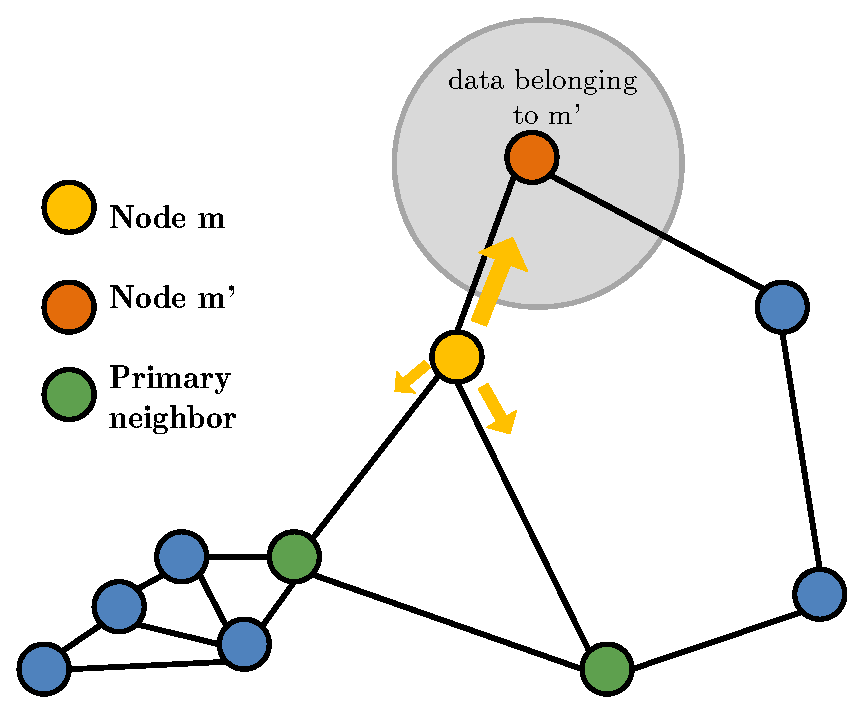
\includegraphics[width=0.6\textwidth]{figures/gsmms/gsmms_update.eps}\\
  \caption{GSMMS inner loop iterative update of $\xi_m$ as described in Step 3}\label{fig:gsmms_update}
\end{figure}
In Step 3 of the update algorithm, the learning rate balances the trade offs
between training sample size, local model fitting error, neighborhood
topology and SOM iteration decay. These factors can be visualized in
Figure~\ref{fig:gsmms_update}. The orange arrows projecting outward from node
$m$ shows directions and magnitudes corresponding to the update vector
${{\alpha _{m'}}\left( {{{\mathbf{\mu}}_{m'}} - {\xi _m}\left( k \right)}
\right)}$. In a highly nonlinear region such as $m'$ , the local PLS model
for $m'$ would have large $\mathrm{MSE}_{m'}$, this results in higher weight being
assigned in the direction of $m'$. 
The higher weight towards $m'$ will draw neighborhood nodes closer, thus compensating for the higher local fitting error.
Similarly, if a local node is assigned many training observations in
its partition, the node will carry heavier weight and attract nearby nodes.
As a result, data-rich regions (in terms of training data availability) will
attract more SOM nodes, leading to finer partitions with better local
prediction.

To improve the computational efficiency, we only apply local updates to PLS models where the $BMU$ membership experienced changes from the previous iteration. Minuscule movements and fine tuning of node location
$\xi_m$ usually do not result in membership changes; therefore, the PLS models do not need to be retrained. This modification
improves the speed of the update step by as much as five times.

\subsection{Network growth mechanism}
After the SOM converges, the global fitting error can be calculated as follows:
\[e_{global} = \nicefrac{\sqrt{\sum\limits_{m = 1}^M {\left( {\sum\limits_{i \in {\bf J_m}}^{} {} {{\left( {{{\hat y}_i} - {y_i}} \right)}^2}} \right)}}}{N} \]

The global fitting error is used to determine if the added SOM node is beneficial. To achieve the most parsimonious model, simpler SOM is preferred unless the added node improves the global fitting error by a predefined threshold (for example, 5\%). 
If the threshold is not exceeded, the outer loop terminates and the SOM training is complete. Otherwise, a new node is added.

Inspired by the GSOM applications in Liu et al. \cite{Liu2009a}, new nodes are inserted around regions with the highest local fitting error (Equation~\ref{eqn:local_error}):
\begin{enumerate}
\item Find the node with the largest $\mathrm{MSE}_m$, call this node $p$
\item Find the furthest node $q$ from its primary neighbors based on
    Euclidean distance of the codebook vectors: $q =
    \mathop{{\rm{argmin}}}\limits_{m'} \left\| {{\xi _p} - {\xi _{m'}}}
    \right\|$, where $m'$ belongs to the set of primary neighbors
\item Insert a new node at the mid-point $\xi_{new} = \frac{\xi_{p} +
    \xi_{q} }{2}$
\item  Connect the new node with neighbors of nodes $p$ and $q$ in the
    adjacency matrix $\mathbb A$
\end{enumerate}
The above procedure is illustrated graphically in
Figure~\ref{fig:gsmms_adding_nodes}, where the 11th node is added and
connected to the surrounding neighbors of nodes $p$ and $q$. After node
addition, the algorithm would return the inner loop to update the SOM
codebook and the local model parameters.

\begin{figure}[!htpb]
  \centering
  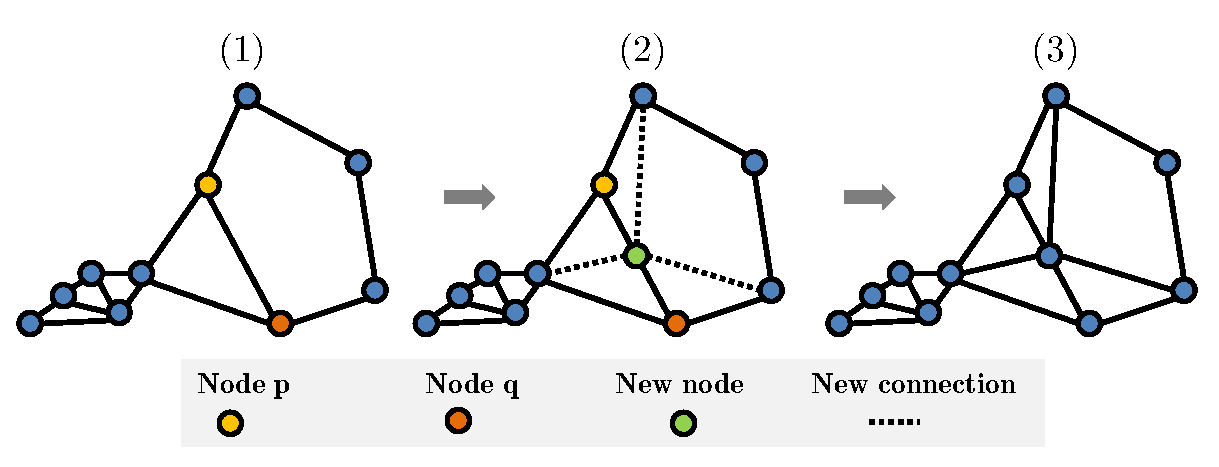
\includegraphics[width=0.95\textwidth]{figures/gsmms/gsmms_adding_nodes.eps}\\
  \caption{Diagram showing GSMMS node insertion into the region with highest local fitting error}\label{fig:gsmms_adding_nodes}
\end{figure}

\added{If the number of nodes in the GSOM network stops increasing, then the GSMMS system has fully converged. In this case, a static GSMMS model is now fully trained and ready for online deployment. However, because both GSOM and PLS models in the GSMMS are static methods, the offline GSMMS system is unable to handle gradual drifts in the process. The next section details the online adaptation mechanisms for the GSMMS to handle process drifts.}

%\subsection{PCA local model modification}
%While the GSMMS framework discussion thus far focuses on prediction models with PLS, this framework can also be adapted to use PCA local models for fault detection and process monitoring.
%
%To train PCA models as local models, a new local and global fitness measure
%needs to be defined. A PCA decomposition gives the following result,
%\[{\bf{X}} = {\bf{\hat X}} + {\bf{\tilde X}} = {\bf{TP}}' + {\bf{\tilde X}}\]
%where $\bf{\hat X , \tilde X}$ are the principal and residual matrices
%respectively. The residual matrix norms are inversely proportional
%to principal matrix norms, where the number of components
%controls the trade-off. Because the number of components for each local model
%is specified to be the same, the residual matrix norm
%$\mathbf{\tilde X}$ is a measure of the local fitting performance. We define
%the local fitting error of node $m$ as the mean Frobenius norm of the
%residual matrix:
%\[{e_m} = \frac{{\left\| {{{{\bf{\tilde X}}}_m}} \right\|}}{{{N_m}}} = \frac{{\sqrt {\sum\limits_{i = 1}^{{N_m}} {\sum\limits_{j = 1}^{{N_m}} {{{\left( {{{\tilde x}_{i,j}}} \right)}^2}} } } }}{{{N_m}}}\]
%
%The global fitting error is defined as the weighted mean of the residual
%matrix norms. The same criteria are applied to ensure that there is
%acceptable improvement (5\%) in global fitting error for the additional node;
%otherwise, the training terminates at the previous SOM structure.
%\[{e_{{\rm{global}}}} = \frac{{\sum\limits_{m = 1}^M {{N_m}{e_m}} }}{N}\]

\section{Online update of GSMMS models}
The GSOM structure allows models to be easily adapted online. The number of nodes and the local models coefficients in the GSOM can be modified at run-time. However, because each node in the GSMMS contains a local PLS model, we need to modify the classical GSOM online adaptation algorithm.

First, the online model update assumes that a trained GSMMS is available. The online update process can be represented as:
\[
\mathrm{GSMMS}_{k+1} = \mathrm{OnlineUpdateFun}(\mathrm{GSMMS}_k, {\bf{S}_{k+1}},{\bf y}_{k+1})
\]
where $k$ is a counter for the number of updates performed, $\mathrm{GSMMS}_k$ is the
total GSMMS parameters at $k$th update. $\bf{s}_{k+1}$ and ${\bf y}_{k+1}$ are the new input features and outputs.

\subsection{Local parameter update}
\begin{figure}
  \centering
  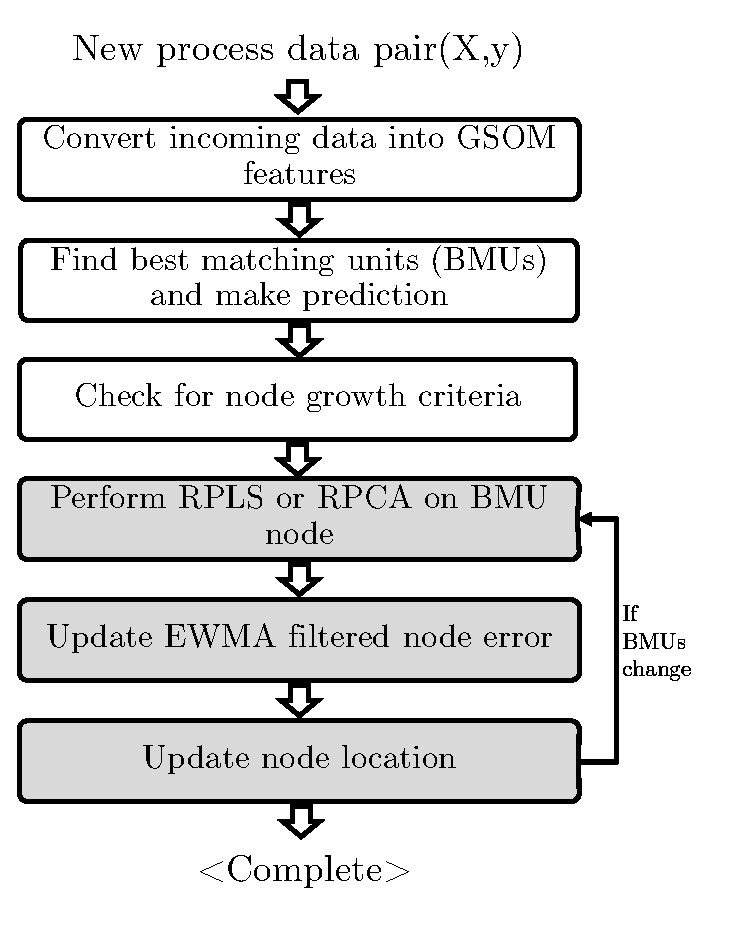
\includegraphics[width=0.55\textwidth]{figures/gsmms/gsmms_model_update.eps}\\
  \caption{GSMMS local parameter update algorithm}\label{fig:gsmms_model_update}
\end{figure}

Figure~\ref{fig:gsmms_model_update} shows the overall steps for GSMMS update. Local model which the new input data activates are updated first. The local model coefficients are updated through recursive PLS \cite{Li2000a,Qin1998}.
Prediction errors for the new feature input are then calculated. Since the original training data is not available during online adaptation, the new prediction errors and the historical prediction errors are combined together using an exponentially weighted moving average filter as follows:
\[e_m^{EWMA}\left( k \right) = \lambda {w_m}\left( {{\bf{s}}\left( k \right)} \right)e_m^{EWMA}\left( {k - 1} \right) + \left[ {1 - \lambda {w_m}\left( {{\bf{s}}\left( k \right)} \right)} \right]\left\| {{e_m}\left( k \right)} \right\|\]
where ${w_m}$ is the Gaussian weighting function specified in Equation~\ref{eqn:gsmms_weight}. The forgetting factor $\lambda$ is tuned to allow the effective sample size of the local node to remain unchanged from the initial training.

The effective sample size is related to the forgetting factor $\lambda$ through:
\[{N_{eff}} = \sum\limits_{k = 0}^\infty  {{\lambda ^k}}  = \frac{\lambda }{{1 - \lambda }},\lambda  \in \left( {0,1} \right)\]

Once the local errors are updated, the codebook vectors of each node are adjusted using a modified version of the codebook update equation based on Equation~\ref{eqn:codebook_update_batch}.
\[{\xi _m}\left( {k + 1} \right) = {\xi _m}\left( k \right) + \tilde \alpha \left( k \right)\left[ {{\bf{s}} - {\xi _m}\left( k \right)} \right], m = 1,2 \ldots M\]
where $\bf s$ is the input feature vector, $\xi_m$ is the codebook of the node being updated, \added{and $\tilde \alpha$ is the recursive learning rate:}

\[
{\tilde \alpha} = \frac{e^{EWMA}_{m'}}{e^{EWMA}_{m'} +{e^{EWMA}_m}} \exp \left( { - \frac{{dis\left({m',m} \right)}}{{2{\sigma ^2}\left( {m'} \right)}}}\right) \exp \left( -\frac{\tau}{\bar{\tau}}\right)
\]
Similar to the batch learning rate $\alpha$, the recursive learning rate
($\tilde \alpha$) is composed of three components:
       \begin{description}
            \item[local error ratio:] $\frac{e^{EWMA}_{m'}}{e^{EWMA}_{m'} +
                {e^{EWMA}_m}}$, this ratio is assigns higher weight to
                regions with higher local fitting error using the EWMA
                filtered error measure.
            \item[topological distance:] $\exp \left( { - \frac{{dis\left(
                {m',m} \right)}}{{2{\sigma ^2}\left( {m'} \right)}}}
                \right)$, the topological distance ensures data from
                neighborhoods further away will have less impact.
            \item[dampening factor:] $\exp \left( -\frac{\tau}{\bar{\tau}}\right)$,
                the $\tau$ is the number of samples assigned to the node being updated, and $\bar{\tau}$ is the average number of samples in all SOM nodes.
        \end{description}

\subsection{SOM structural parameter update}
The recursive update rules adapt the local model coefficients and the locations of nodes. 
However, during scenarios where abrupt changes occur and none of the local model is able to fit the new inputs well, the local parameter updates do not perform well. 
New node needs to be inserted near regions with the highest fitting error.
Two node insertion ways were discussed here for online implementation; these node
insertion all follow the same general principles that were applied
during batch training.

The first method is to compare the incoming prediction error for the new inputs against the EWMA filtered average node errors. An excessive error would indicate that the current nodes are not able to predict the more recent data, and therefore, a new node is required. If there is an significant
improvement in reducing the prediction error, then the new network structure
is kept.

The second node addition heuristic is based on the quantization error of new feature inputs
from the existing GSOM. This is an efficient calculation
since the quantization errors are already computed during the assignment of the BMU for prediction.
If the quantization error exceeds a pre-defined threshold (i.e. 95\% percentile of quantization error), 
a new node can be inserted using similar logic as the offline training case.


\section{Prediction using GSMMS}
\deleted{Local model predictions for multiple model systems faces several challenges: model performance varies depending on availability of training data and the correlation with output in the specific region.
Transitions between local model regions also experience discontinuities due to its discrete nature and sometimes causes erroneous predictions.}

In the proposed GSMMS framework, the general steps to calculate the final predicted output is shown in a process shown in Figure~\ref{fig:gsmms_prediction}. The final output is a weighted average of the local model predictions of the best neighborhood of the incoming data. The best neighborhood is defined as the BMU node of the incoming inputs and its immediate primary neighbors (nodes with direct connection to the BMU node). To combine the predictions of the best neighborhood models, the weight average $\hat y$ is calculated as follows:
\[
\hat y = \nicefrac{{\sum\limits_{i = 1}^I {{w_i}{{\hat y}_i}} }}{{\sum\limits_{i = 1}^I {{w_i}} }}
\]
where
\[
{w_i} = \exp \left( { - \frac{{dis\left( {m,i} \right)}}{{2{\sigma ^2}\left( k \right)}}} \right)
\]




\begin{figure}[!htpb]
  \centering
  % Requires \usepackage{graphicx}
  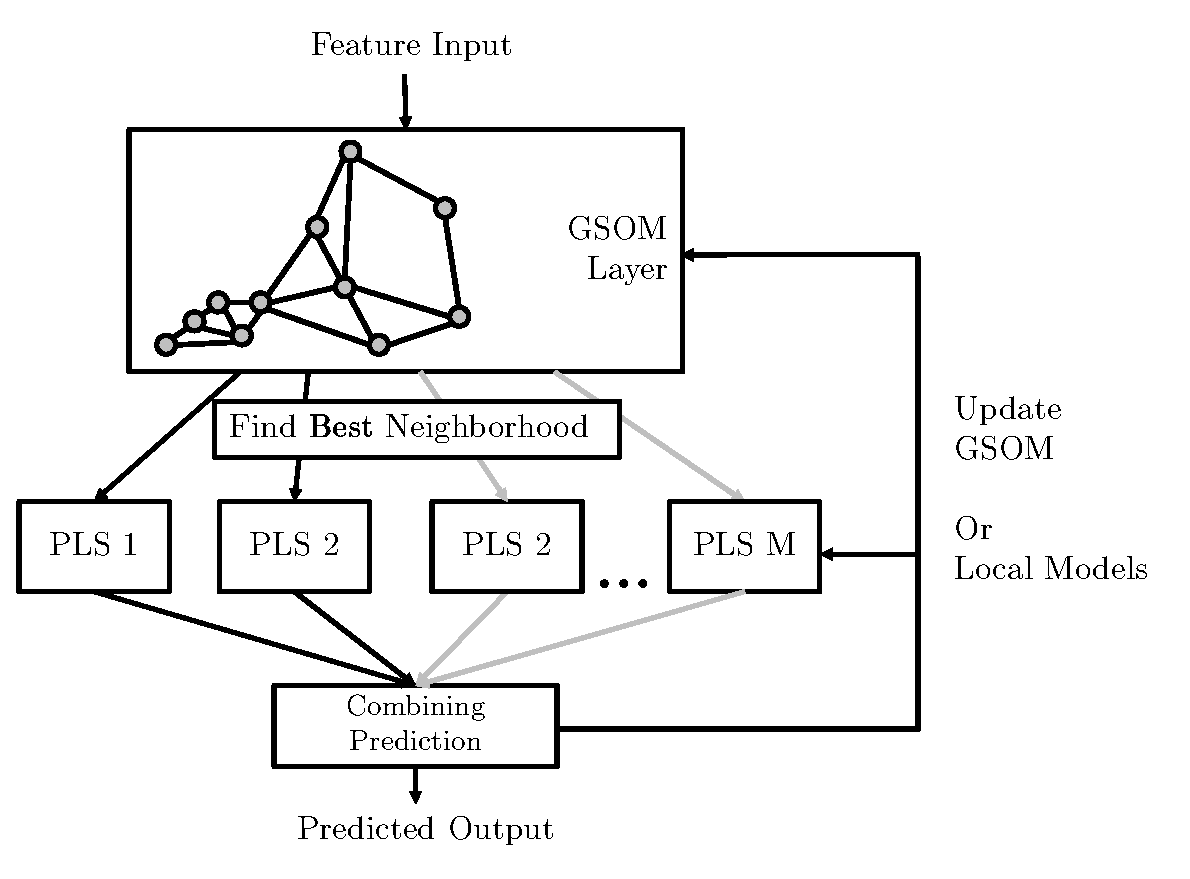
\includegraphics[width=0.95\textwidth]{figures/gsmms/gsmms_prediction.eps}\\
  \caption{Schematic of the prediction and the online adaptation of proposed GSMMS framework}\label{fig:gsmms_prediction}
\end{figure}

\clearpage
\section{Simulated test cases}
Three test cases were performed using simulation to demonstrate the
effectiveness of proposed method:
\begin{enumerate}
\item Input-output data from five different states with clear separation in the input space between each state
\item Input-output data with nonlinear relationship
\item Input-output data from five different states with overlapping boundaries in the input space
\end{enumerate}

In these test cases, we simulate a multi-modal process with 10 inputs and 1 output. \added{The inputs are generated from a linear combinations of latent noise series as follows:}
\[
\mathbf X_i = \mathbf V \mathbf T_i^T + \mathbf E_{\mathrm input}
\]
where $\mathbf X_i \in \mathbb{R}^{(N_i \times 10)}$ is the input in mode $i$, $\mathbf T_i \in \mathbb{R}^{(10 \times P)}$ is a randomly generated loading matrix for each mode $i$, $\mathbf V_i \in \mathbb{R}^(N_i \times P)$ is a sampled subset ($N_i$ elements) of the latent noise series, and $\mathbf E_{\mathrm input} \sim \mathcal{N}(\mu_{input},\,\sigma_{input}^{2})\,$ is the additive Gaussian noise. The latent noise series are sampled from an existing industrial dataset under steady-state operating conditions; we found this to give more realistic simulated data than simply using a random walk noise series as the underlying input. The final output is generated as a linear combination of the inputs with additive white noise as follows: 
\[
\mathbf y_i = \mathbf X_i \mathbf B_i + E_{\mathrm output}
\]
where $y_i \in \mathbb{R}^{(N_i \times 1)}$ is the output of mode $i$, $\mathbf B_i \in \mathbb{R}^{(10 \times 1)}$ is the linear coefficients for mode $i$, and $\mathbf E_{\mathrm output} \sim \mathcal{N}(\mu_{output},\,\sigma_{output}^{2})\,$ is the additive output Gaussian noise.
The above calculation is repeated $I$ times, where $I$ is the number of modes specified. 

While this system does not simulate the dynamic behavior during state transitions, it represents a typical set of input-output data for continuous steady-state systems.

15,000 samples are simulated in the dataset. 5,000 samples are used as
training data and the other 10,000 are used as testing data.
The initial GSOM feature inputs uses the first three component scores from a global PCA model, while the local model inputs still use the full input space. 
This global PCA model captures 85\% of the total variance in the process inputs.

Figure~\ref{fig:gsmmsfig1a} lists the GSOM diagnostics of a model just after
initialization, the top plot is the number of training samples belonging to each node (number of activations) and the bottom plot shows the root-mean-squared error of each node. 
The node locations were initialized randomly and the local node errors were calculated
using the membership association at the time of initialization.
Figure~\ref{fig:gsmmsfig1b} shows the first two principal component scores of the GSOM for better visualization.
\begin{figure}[htpb]
  \centering
  \subfigure[GSOM node activation and error]{
    \includegraphics[width=0.45\textwidth]{figures/gsmms/figure1a.eps}
    \label{fig:gsmmsfig1a}
  }
  \subfigure[GSOM codebook location and training inputs]{
    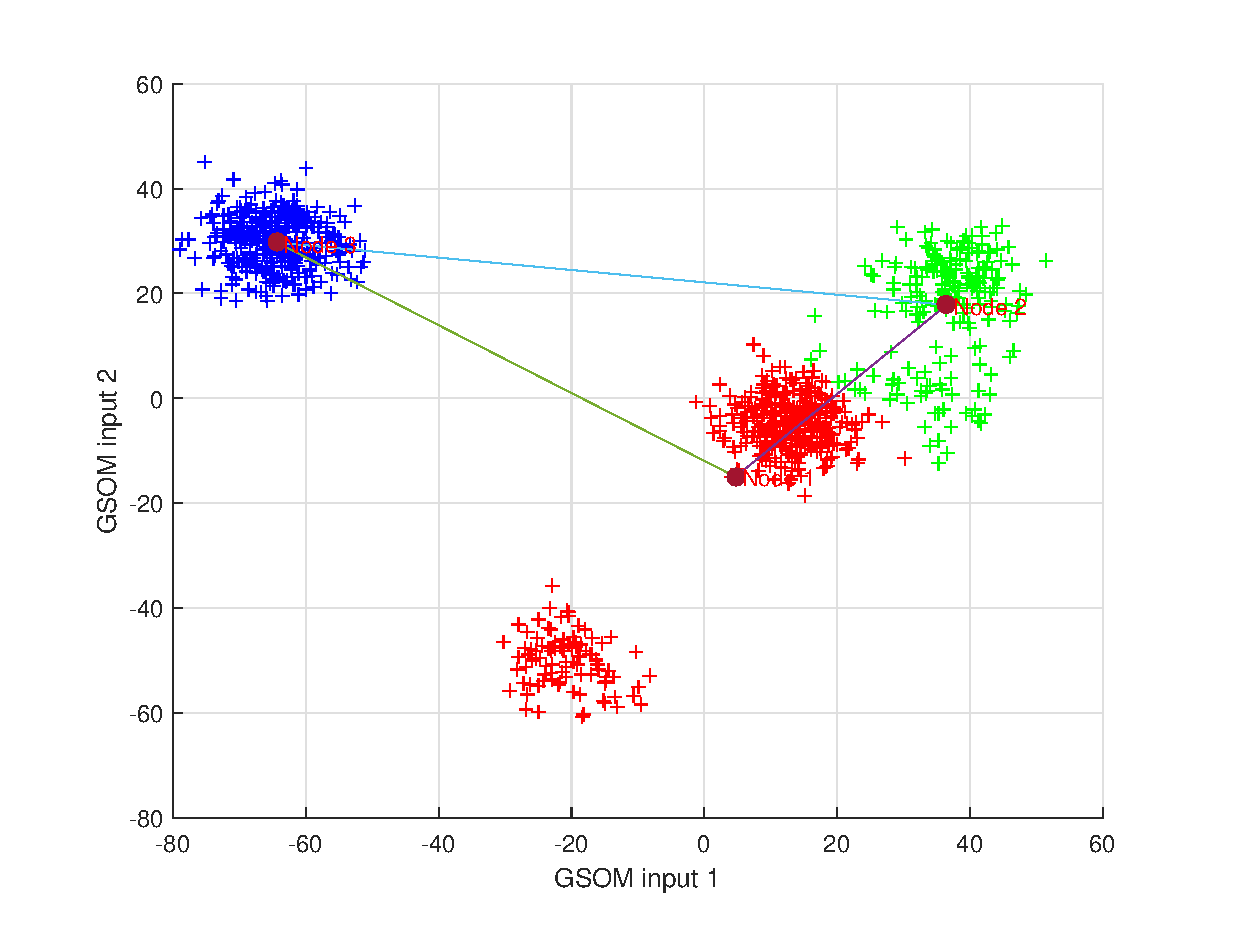
\includegraphics[width=0.45\textwidth]{figures/gsmms/figure1b.eps}
    \label{fig:gsmmsfig1b}
  }
  \caption{GSOM node error and codebook location after initialization}
  \label{fig:gsmmsfig1}
\end{figure}

After the GSOM undergoes batch offline training, the structural parameters
and the diagnostics are shown in Figure~\ref{fig:gsmmsfig2}.
The trained model contains five nodes, which corresponds to the true number of operating modes in simulation.
In addition, the number of activation and the root-mean-squared error of each node are
inversely correlated; nodes with the highest number of activation have lower
root-mean-squared error. This implies that GSOM attempted to assign more data to nodes with better prediction performance.

\begin{figure}[htpb]
  \centering
  \subfigure[GSOM node activation and error]{
    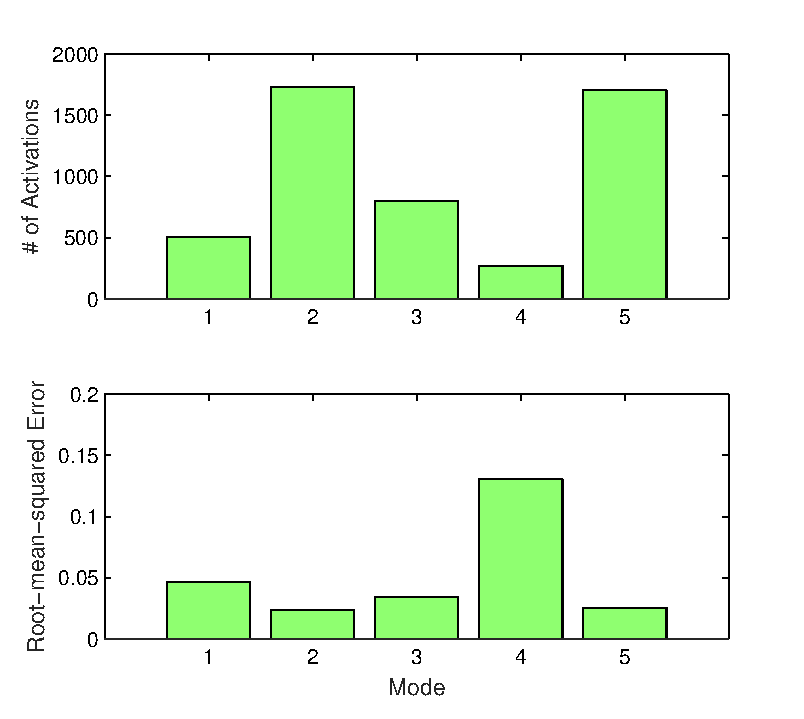
\includegraphics[width=0.45\textwidth]{figures/gsmms/figure2a.eps}
    \label{fig:gsmmsfig2a}
  }
  \subfigure[GSOM codebook location and training inputs]{
    \includegraphics[width=0.45\textwidth]{figures/gsmms/figure2b.eps}
    \label{fig:gsmmsfig2b}
  }
  \caption{GSOM node error and codebook coordinates after training has been completed}
  \label{fig:gsmmsfig2}
\end{figure}

Figure~\ref{fig:gsmmsfig3} shows the testing dataset mapped onto the trained
SOM. Since this simulated data did not include a drifting disturbance, the
model is able to accurately predict the results with a $R^2$ value of 0.91.

\begin{figure}[htpb]
  \centering
  \subfigure[Testing dataset score plot]{
    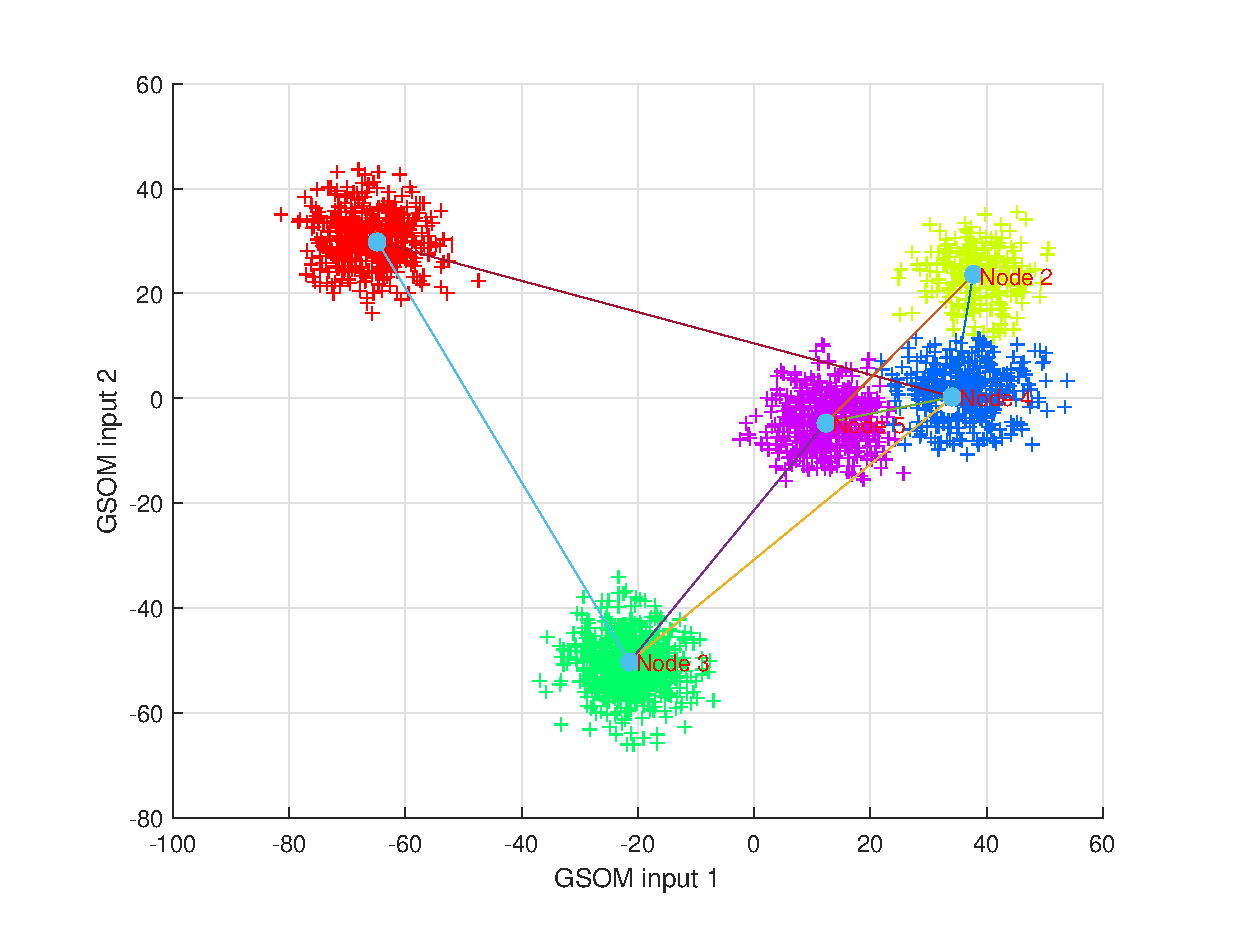
\includegraphics[width=0.45\textwidth]{figures/gsmms/figure3a.eps}
    \label{fig:gsmmsfig3a}
  }
  \subfigure[Predicted and actual values of the testing dataset]{
    \includegraphics[width=0.45\textwidth]{figures/gsmms/figure3b.eps}
    \label{fig:gsmmsfig3b}
  }
  \caption{Testing data score plot and the GSOM model predictions}
  \label{fig:gsmmsfig3}
\end{figure}

In the second test case, we introduce some simple nonlinearity into the simulation as follows:
\[y = {\beta _1}\exp \left( { - {x_1}/{x_2}} \right) + {\beta _2}{x_3}{x_4} + {\beta _3}{x_5}^2 + {\beta _4}{x_6} + {\beta _5}{x_7} + {\beta _0} + \varepsilon \]

The input and the generated output are plotted in Figure\ref{fig:gsmmsfig4a}.
The trained network structure is shown in Figure~\ref{fig:gsmmsfig4b}, and
the final testing prediction is shown in Figure~\ref{fig:gsmmsfig4c}.
In this case, the GSOM optimized to a five node network to better
approximate the nonlinearity in the system. The prediction performance on the
testing dataset resulted in a $R^2$ value of 0.81.

\begin{figure}[htpb]
  \centering
  \subfigure[Simulated inputs and nonlinear output time series plot]{
    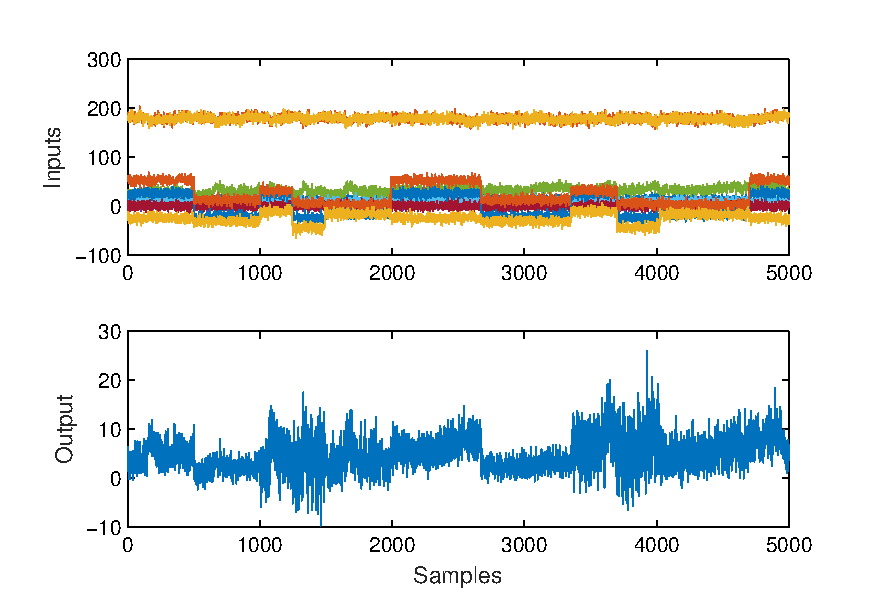
\includegraphics[width=0.45\textwidth]{figures/gsmms/fig4a.eps}
    \label{fig:gsmmsfig4a}
  }
  \subfigure[SOM network structure after training]{
    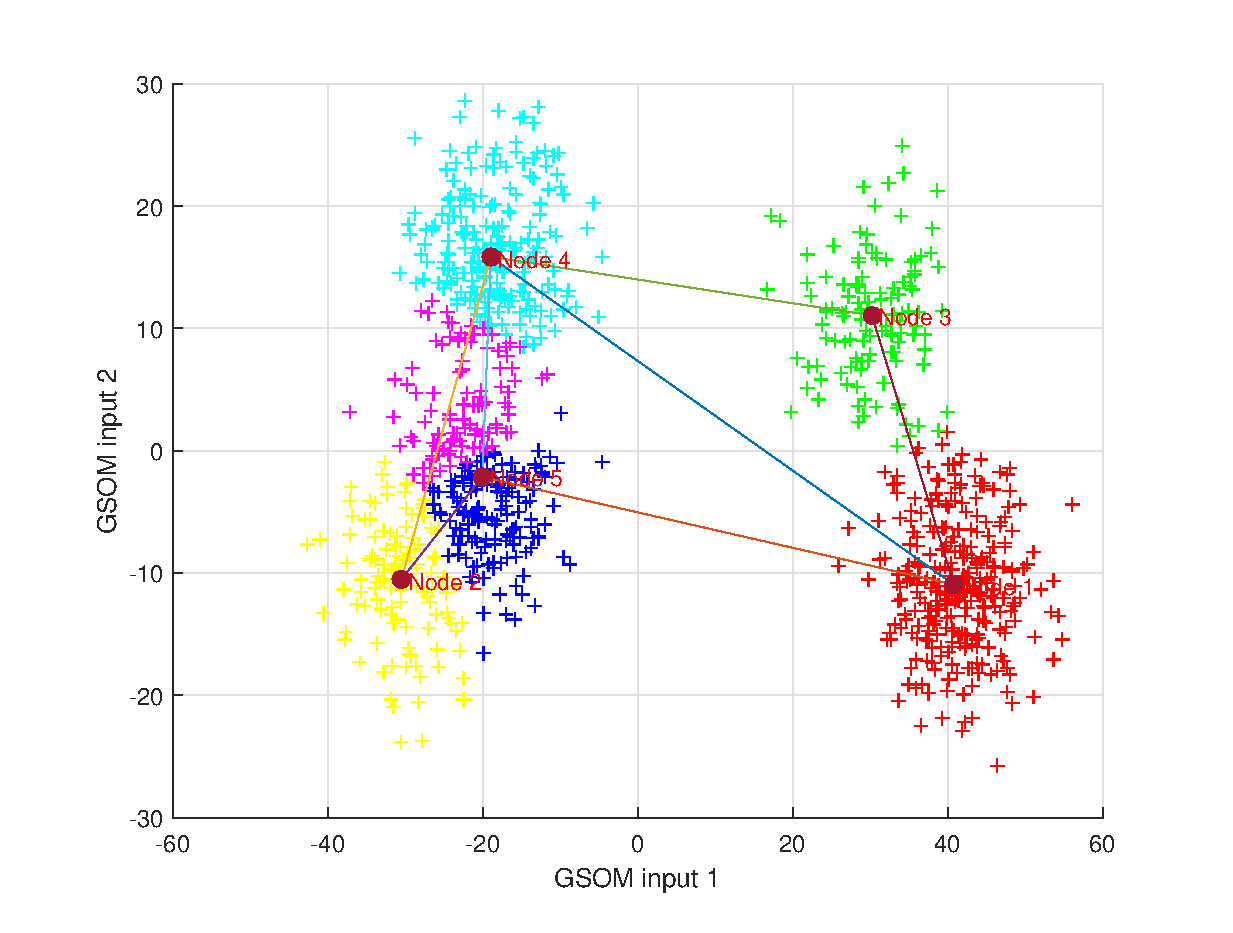
\includegraphics[width=0.45\textwidth]{figures/gsmms/fig4aa.eps}
    \label{fig:gsmmsfig4aa}
  }
  \subfigure[GSOM diagnostics information]{
    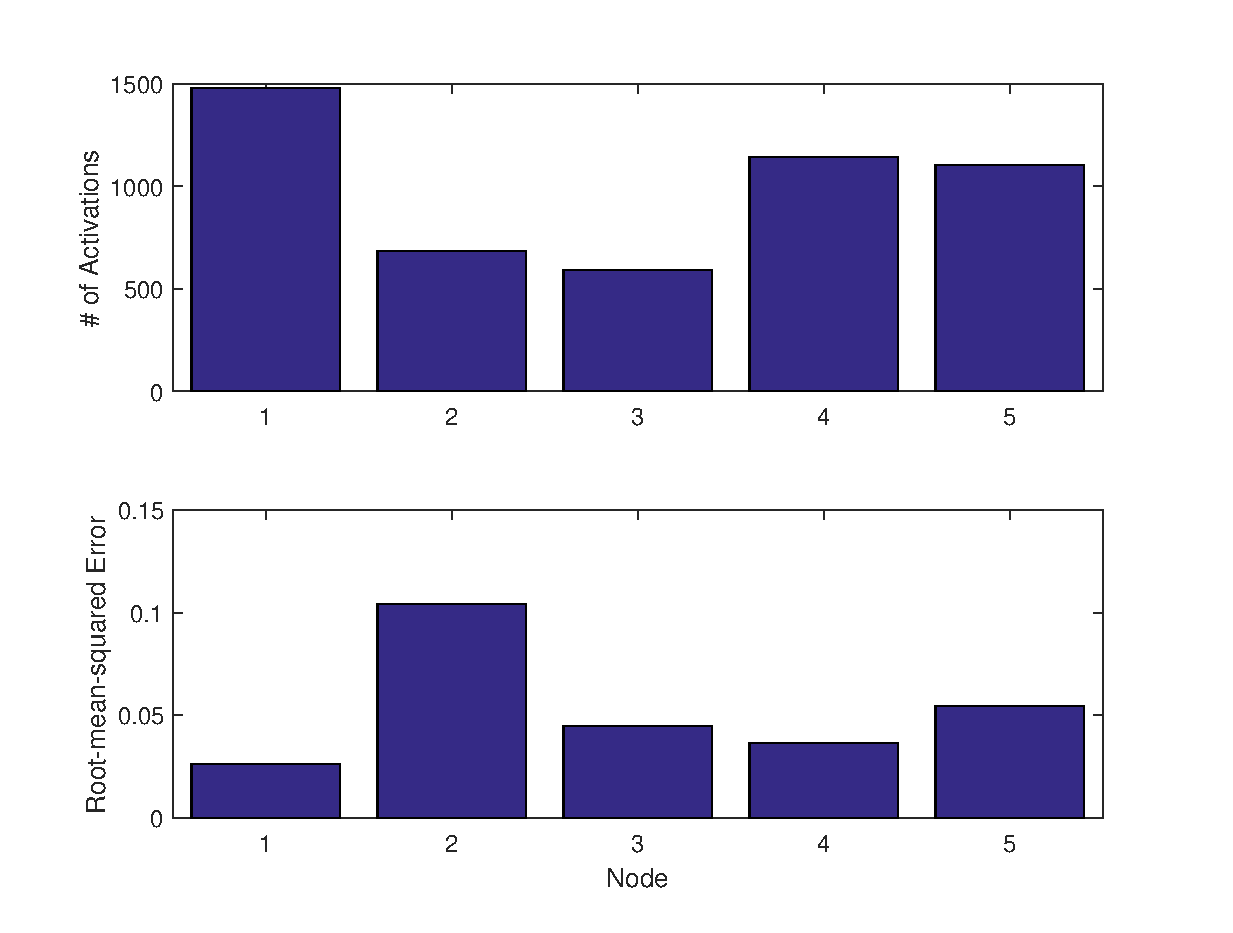
\includegraphics[width=0.45\textwidth]{figures/gsmms/fig4b.eps}
    \label{fig:gsmmsfig4b}
  }
  \subfigure[Predicted and measured outputs for the testing dataset]{
    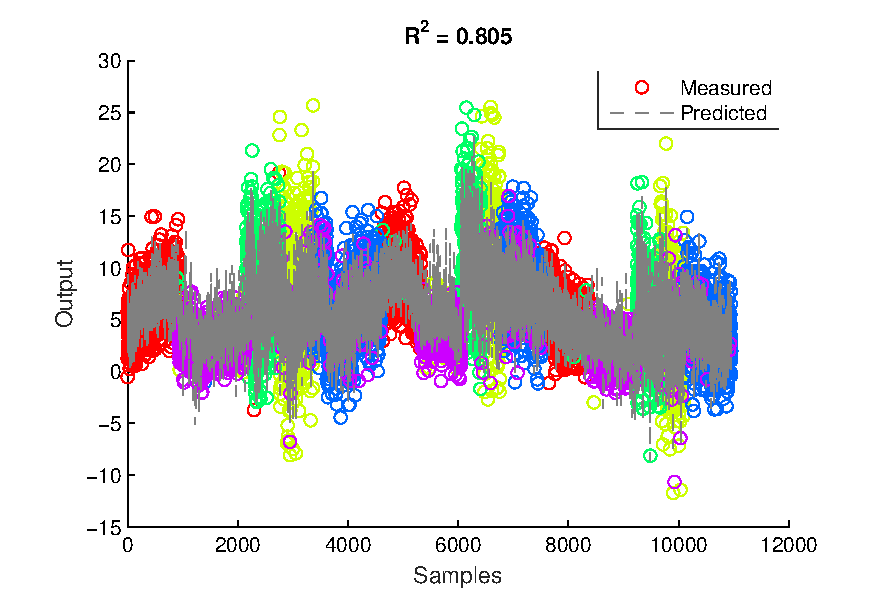
\includegraphics[width=0.45\textwidth]{figures/gsmms/fig4c.eps}
    \label{fig:gsmmsfig4c}
  }
  \caption{Training and testing results of nonlinear simulated case study}
  \label{fig:gsmmsfig4}
\end{figure}

The third test case simulates scenarios with significant operating mode overlap.
The boundary overlaps are simulated by reducing the variance in the model inputs across operating modes.
As a result, the operating mode boundaries are blended together and difficult to separate, increasing the difficulty for multiple model systems. 
The GSMMS trained network structure and the simulated input data are shown in Figure~\ref{fig:gsmmsfig5}.
The trained GSMMS network arrived at a node size of six (greater than five modes used in simulation).
The finer partition allows the GSMMS model to isolate regions of high overlap and improve on prediction in regions with less overlap.

The prediction, training coefficient of determination ($R^2$) and prediction
errors are tabulated in Table~\ref{tab:gsmms_simulated}. Performances of two additional model are also shown as benchmarks. The baseline model represents the current industrial practice of assuming contiguous blocks of training data from a single operating mode and creates only a single PLS model.
The ideal case assumes perfect knowledge about the operating mode information and creates a PLS model for each separate mode based on the true operating mode information.
The GSMMS model behaves close to the ideal case performance for cases 1 and 2.
In case 3 with excessive data overlap, the GSMMS suffers a drop in prediction performance, but it is
still performing better than single mode models.
As a result, the multiple model system approach is superior if the development process can be
simplified and streamlined for practical use in industrial applications.

\begin{figure}[htpb]
  \centering
  \subfigure[Score plot of the training data]{
    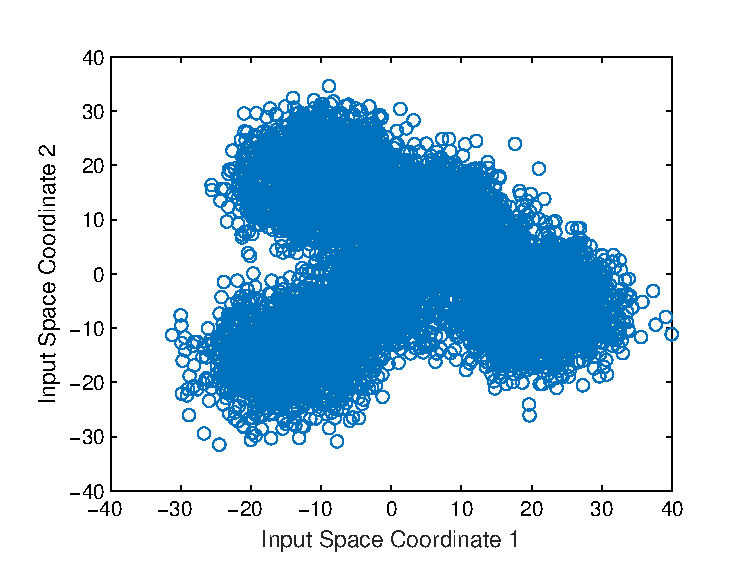
\includegraphics[width=0.45\textwidth]{figures/gsmms/fig5a.eps}
    \label{fig:gsmmsfig5a}
  }
  \subfigure[SOM partitioning of the input space]{
    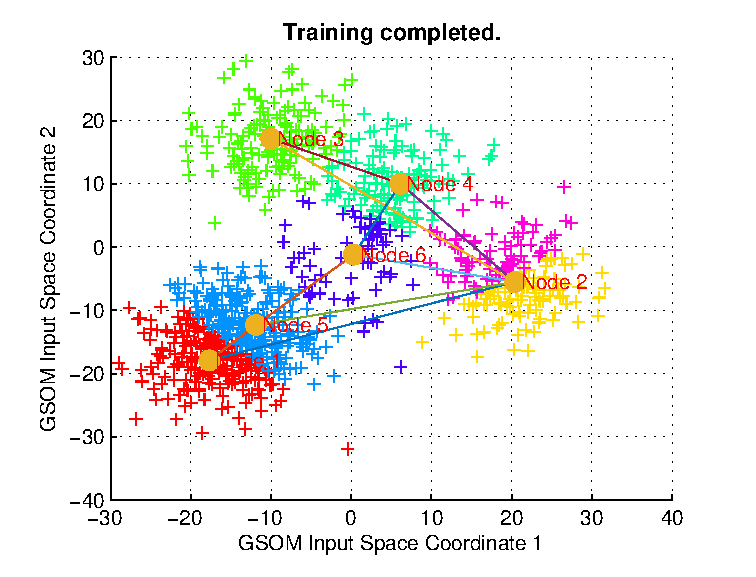
\includegraphics[width=0.45\textwidth]{figures/gsmms/fig5b.eps}
    \label{fig:gsmmsfig5b}
  }
  \caption{Score plot and GSOM structure diagram for the case with overlapping operating modes}
  \label{fig:gsmmsfig5}
\end{figure}


\begin{table}[htbp]
  \centering
  \caption{Prediction performance of the GSMMS framework in three simulated case studies}
  \footnotesize
      \begin{tabular}{rccc}
    \toprule

          \textbf{Model } & \textbf{\# of Nodes} & \textbf{Testing R2 } & \textbf{RMS Error } \\
    \midrule
        & \multicolumn{3}{c}{Case 1 - Operating Mode with Clear Separation} \\
    \midrule
    Ideal case  & 4     & 0.97  & 1.01 \\
    Baseline & 1     & 0.7   & 3.04 \\
    Piecewise GSMMS  & 4     & 0.97  & 1.01 \\

          & \multicolumn{3}{c}{Case 2 - Multiple Operating Mode with Nonlinear Output} \\
    \midrule
    Ideal case  & 4     & 0.98  & 0.99 \\
    Baseline & 1     & 0.76  & 3.53 \\
    Piecewise GSMMS  & 5     & 0.91  & 2.38 \\

          & \multicolumn{3}{c}{Case 3 - Multiple Operating Modes with Overlapping Modes} \\
    \midrule
    Ideal case  & 5     & 0.96  & 1.09 \\
    Baseline & 1     & 0.52  & 4.23 \\
    Piecewise GSMMS  & 6     & 0.85  & 2.13 \\
    \bottomrule
    \end{tabular}%
  \label{tab:gsmms_simulated}%
\end{table}

\clearpage

%\input{section-temex.tex}

\newpage
\section{Industrial Case Study}
Plasma etching \cite{Plummer2000} is an unit operations commonly used in semiconductor manufacturing. Figure~\ref{fig:plasma_etcher} shows a schematic of a plasma etch reactor.
Ionized etchant gases (usually fluorine, chlorine based, halide containing species)
reacts physio-chemically with the surface silicon. Figure~\ref{fig:plasma_etch} illustrates the different etching mechanisms that are simultaneously present. Isotropic etching could cause undercutting, while physical sputtering could cause trenching; both of which are undesirable
outcomes. To mitigate these effects, the trim time for the etch step has to
be controlled precisely, which requires an accurate process model.

In gate etching processes, line-width profiles and critical dimension are
critical parameters that correlate to the performance of the final device.
Metrology stations are used to measure these quality parameters before and
after gate etch to ensure wafer quality. These metrology measurements are
illustrated in Figure~\ref{fig:metrology_examples}.

\begin{figure}[!htpb]
  \centering
  \includegraphics[width=0.9\textwidth]{figures/intro/plasma_etcher.png}\\
  \caption{Schematic of a typical plasma etching system}
  \label{fig:plasma_etcher}
\end{figure}

\begin{figure}[!htpb]
  \centering
  \includegraphics[width=0.8\textwidth]{figures/intro/plasma_etch.png}\\
  \caption{Summary of etching mechanisms and typical problems in plasma etching}
  \label{fig:plasma_etch}
\end{figure}


\index{Gate etch}%
\index{FICD}%
\index{FICD!Final Inspection Critical Dimension}%
\index{DICD}%
\index{DICD!Develop Inspection Critical Dimension}%


\begin{figure}[!htpb]
  \centering
  \includegraphics[width=0.8\textwidth]{figures/application/metrology_meas.png}\\
  \caption{Transmission Electron Micrograph (TEM) of a polysilicon gate geometry showing the quality variables of interest}\label{fig:metrology_examples}
\end{figure}

The gate etch dataset contains 1800 wafers with metrology measurements of Develop-Inspect Critical Dimension of the resist pattern (DICD) and Final Inspect Critical Dimension
(FICD). Modeled outputs could be expressed as either the difference between
these measurements (etch bias) or the etch bias divided by the trim etch time
as the etch rate. This study attempts to predict the etch rate from the various process inputs of the etch tool. Figure~\ref{fig:raw_data_3} shows the etch rate of the entire dataset.
The first 205 wafers are used as training data; the rest of the dataset
are used for validation and testing.

The process inputs are collected through the fault detection and classification (FDC) system of the tool. 
The FDC measurements contain instrument read-outs from the RF circuitry, etchant gas flow
, chamber temperature, vacuum systems, and various spectroscopic sensors. The data collection rate is 0.5 Hz. Additional contexet information such as recipe step, process
time and EWMA-estimated disturbances in the controller are also available. In total, batch trajectories from 39 measurements were used as input
variables. An example plot of the raw trace data is shown in Figure~\ref{fig:raw_data}.

\begin{figure}[!htpb]
\centering
\subfigure[]{
  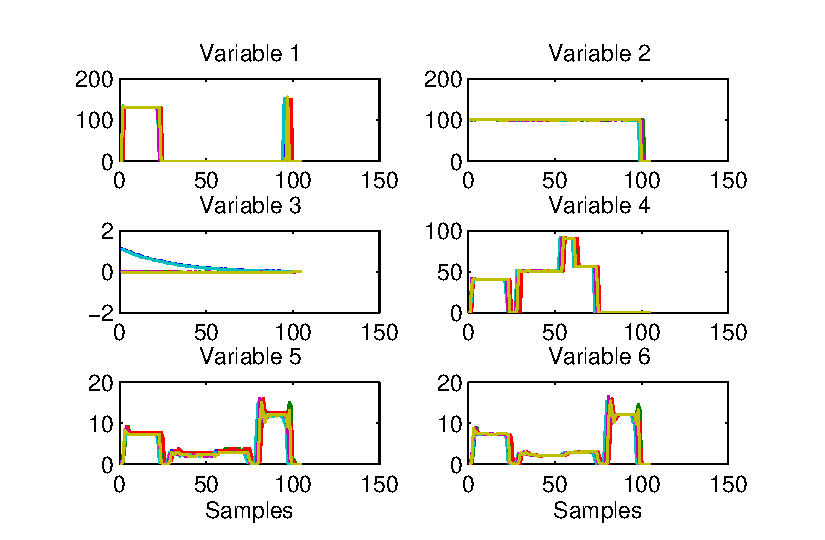
\includegraphics[width=0.45\textwidth]{figures/application/fig_raw_data_1.eps}
    \label{fig:raw_data_1}
}
\subfigure[]{
  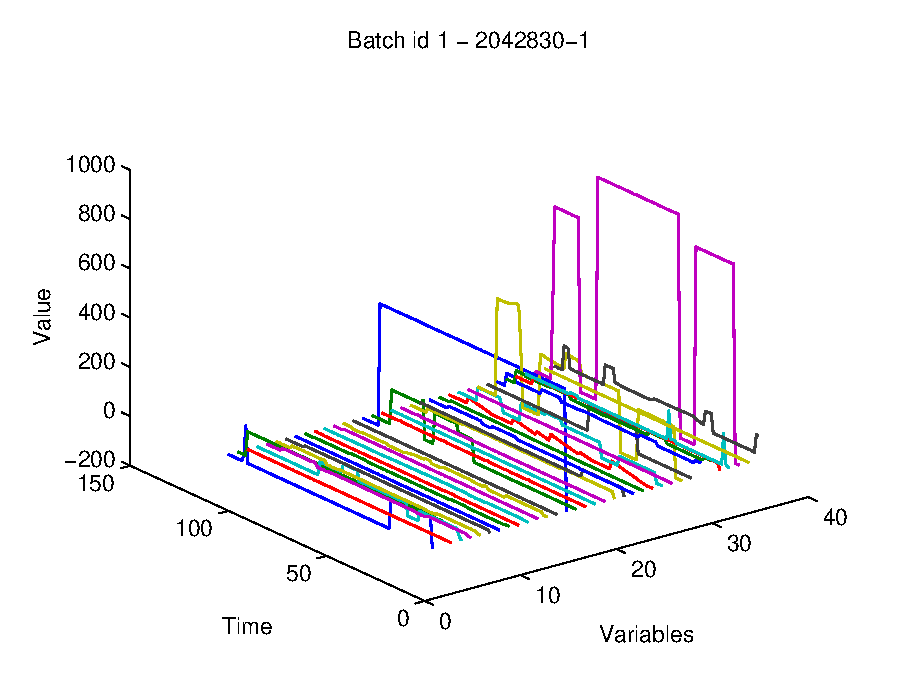
\includegraphics[width=0.45\textwidth]{figures/application/fig_raw_data_2.eps}
    \label{fig:raw_data_2}

} \subfigure[]{
  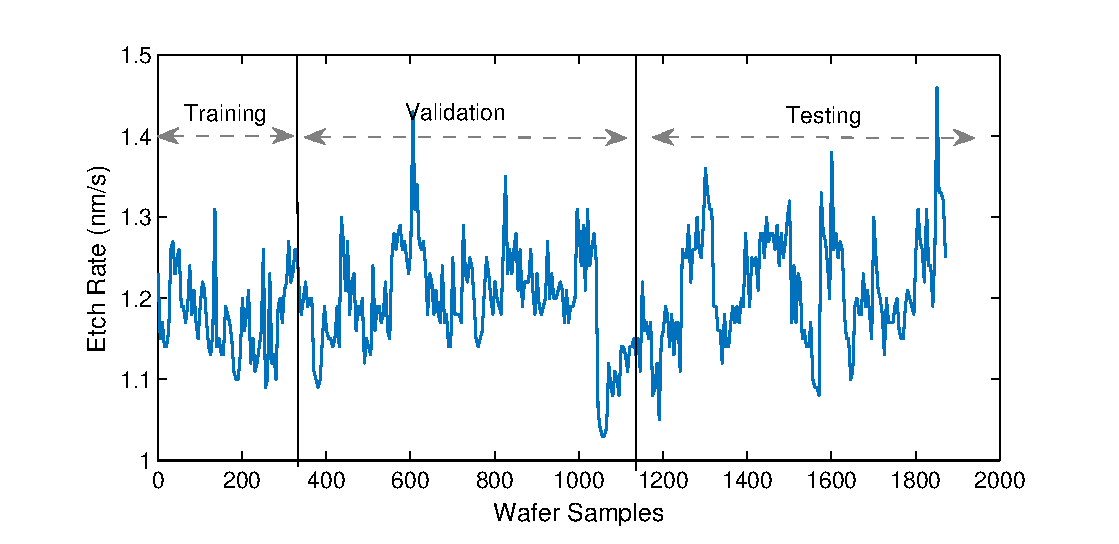
\includegraphics[width=0.95\textwidth]{figures/application/fig1_output_raw.eps}
    \label{fig:raw_data_3}
} \caption[raw data plot]{Raw data plot showing \subref{fig:raw_data_1} the
temporal profiles of six variables for five wafer batches,
\subref{fig:raw_data_2} A three-dimensional representation of trajectories
from a single batch, and \subref{fig:raw_data_3} output variable etch rate}
\label{fig:raw_data}
\end{figure}

\clearpage
\subsection{Data Pretreatment}
Missing and redundant data, empty rows and columns are first removed from the dataset. 
Temporal outliers such as spikes in sensor readings were also removed.
After initial cleaning, the dataset was then unfolded into a 2-D array using
batch-wise unfolding \cite{Westerhuis1999}. Batch-wise outliers were then removed from the unfolded data. Additional data sanitation checks utilizing process knowledge were also carried out. For example, batches where there are significant trajectory deviations in the recipe step were removed. After initial trajectory screening, the trajectories were then aligned using
robust-derivative dynamic time warping \cite{Zhang2013} based on the
indicator variable ``recipe number''. Univariate scaling and mean-centering
were then applied to the unfolded input-output data to create the
$\mathbf{X}$ and $\mathbf Y$ matrices.


\subsection{GSMMS with PLS local model}
A GSMMS model with local PLS models was trained for this data
set. The resulting unfolded multi-way dataset contains approximately 650
inputs. 
The feature input into the GSOM consisted of the first three principal component scores of the PCA projection of the unfolded training data. 
Initial offline batch training produced a 5 node GSOM network; its network structure and the feature inputs (first two PCA scores) are plotted in Figure~\ref{fig:gate_etch_gsmms_training}.
The scores show a parabolic shape for the training inputs, indicating that there is strong non-steady-state operation in the process. 

To simulate online adaptation, the GSMMS model was updated batch-wise for every five wafers. The most recent GSMMS model was used for prediction (from 1-step ahead to 5 step-ahead). The resulting network structure after iterating through the entire testing data is shown in
Figure~\ref{fig:gate_etch_gsmms_testing}. Comparing against the offline trained GSOM, the network size has increased to 6 nodes. We also observe an increased density of nodes around the left
``tail'' of the parabola. This indicates that particular region had higher activation rates in the more recent data. The prediction performance of the adaptive GSMMS is plotted in
Figure~\ref{fig:gate_etch_gsmms_prediction}. The adaptive GSMMS was able to successfully track the measured etch rate across two maintenance events (around sample 220 and sample 800). The GSMMS performance was also compared against several benchmark methods in Table~\ref{tbl:final_comparison}.


\begin{figure}[!htpb]
  \centering
    \subfigure[]{
    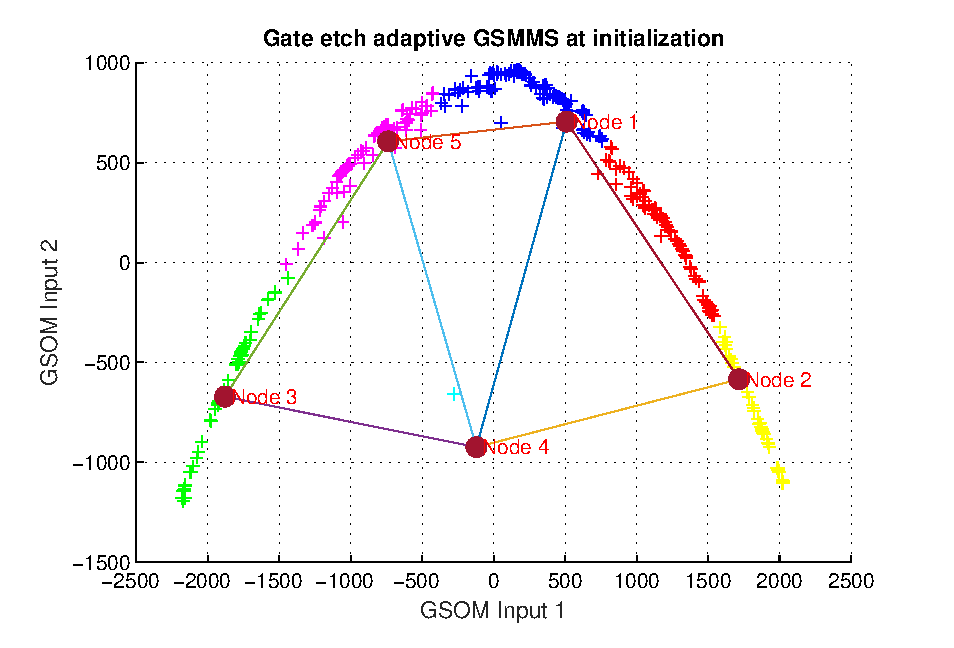
\includegraphics[width=0.45\textwidth]{figures/application/gate_etch_gsmms_training.eps}
    \label{fig:gate_etch_gsmms_training}
    }
  \subfigure[]{
    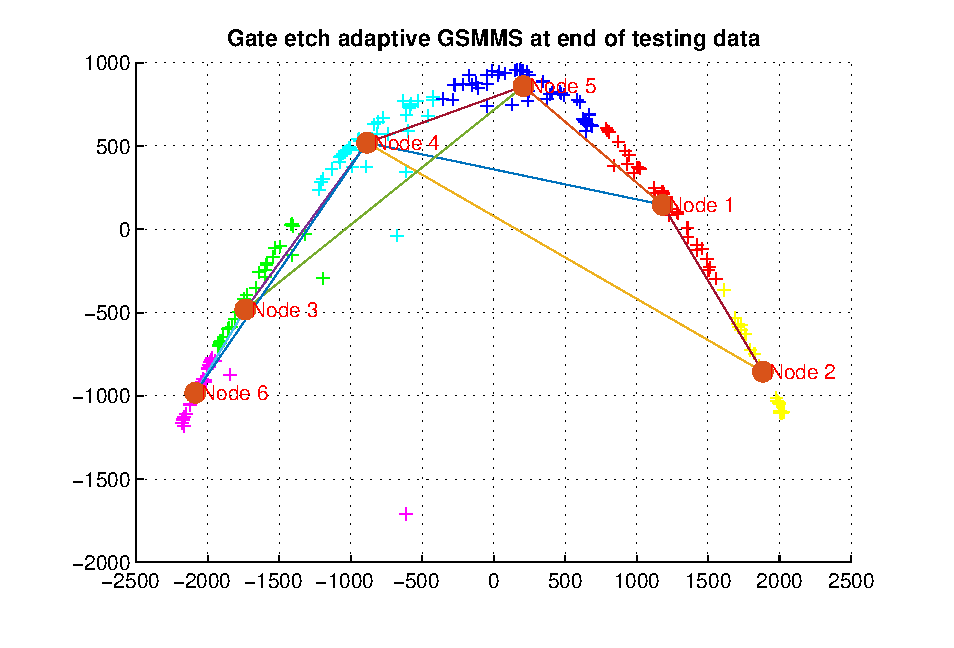
\includegraphics[width=0.45\textwidth]{figures/application/gate_etch_gsmms_testing.eps}
    \label{fig:gate_etch_gsmms_testing}
    }
  \caption{Gate Etch adaptive GSMMS \subref{fig:gate_etch_gsmms_training} post-training and \subref{fig:gate_etch_gsmms_testing} final (after testing data update) network structure}\label{fig:gate_etch_gsmms}
\end{figure}

\begin{figure}
  \centering
  % Requires \usepackage{graphicx}
  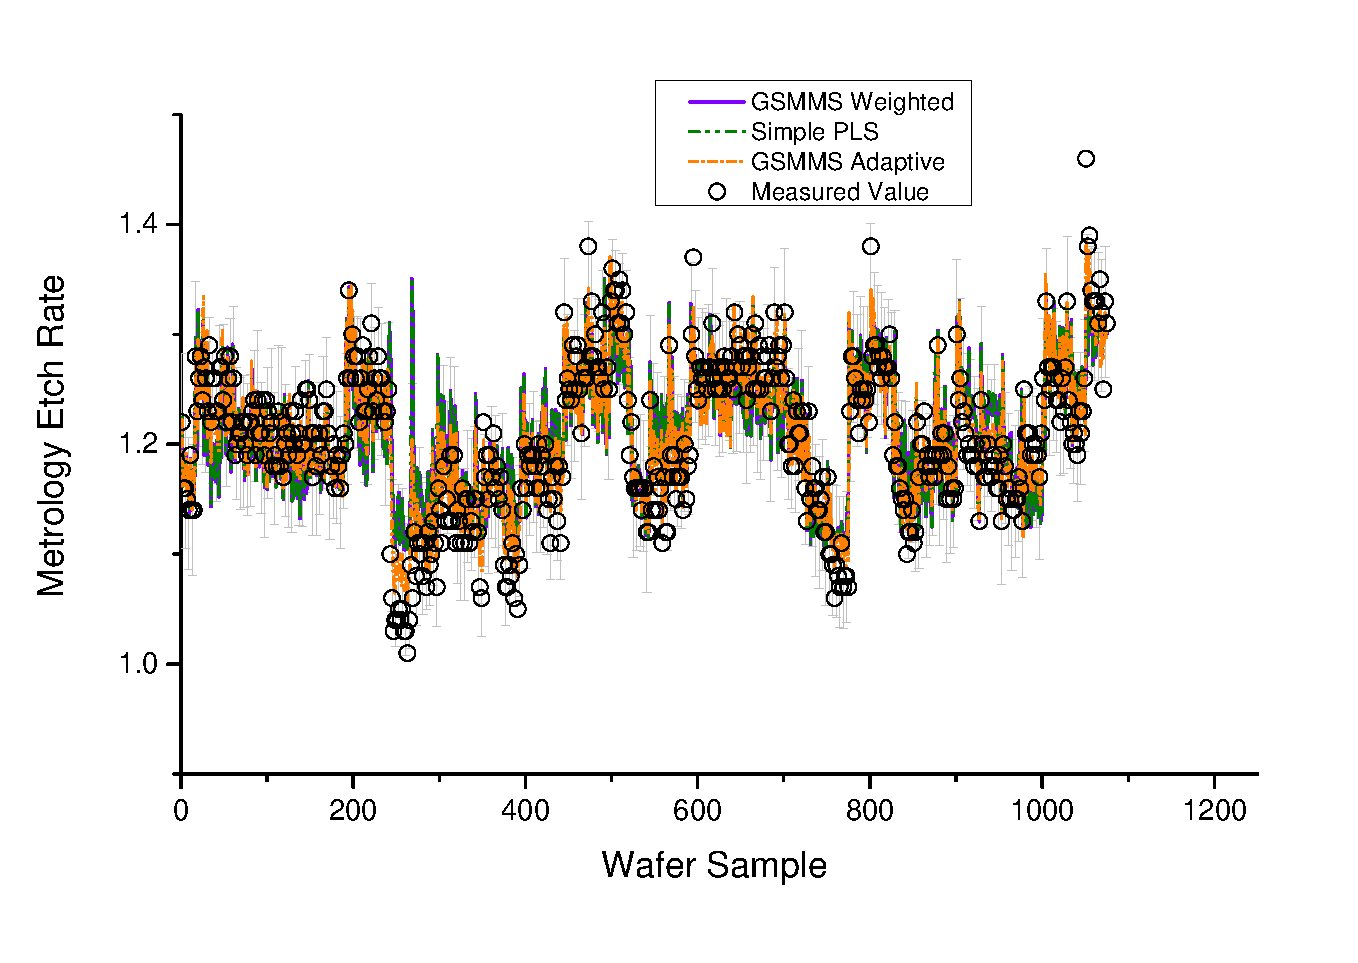
\includegraphics[width=0.95\textwidth]{figures/application/gate_etch_gsmms_prediction.eps}\\
  \caption{Prediction results of the Adaptive GSMMS model for the testing dataset}\label{fig:gate_etch_gsmms_prediction}
\end{figure}

\clearpage

\begin{table}[htpb]
\centering
\caption {Model size, coefficient of determination, and cross-validated root mean squared residual of candidate models}
\footnotesize
    \begin{tabular}{lccc}
    \toprule
       Method                               &    Approx. model size &  Testing $R^2$ & RMS residual \\ \hline
       PCA regression &    2700          & 0.425               & 0.0495     \\
       BPNN    &       $2700\times N_{layers}$    & 0.72 / 0.32 &  0.0823 \\
       Nonlinear PLS with Neural networks & $600 \times A \times N_{layers}$ & 0.56 / 0.25                          & 0.0623      \\
       Static PLS &    600          & 0.142              & 0.0998     \\ \hline
       MW-PLS &    600          & 0.442              & 0.0598     \\
       MW-PLS w/ TPLS&    ~600          & 0.66              & 0.029     \\
       Adaptive GSMMS-PLS &    $600 \times 5\rightarrow 600 \times 6 $          & 0.812              & 0.019     \\
       \bottomrule
    \end{tabular}
    \label{tbl:final_comparison}
\end{table}

\begin{table}[htpb]
\centering
\caption {Qualitative evaluation of the candidate models and their implementation difficulty}
    \label{tbl:final_comparison2}
\footnotesize
\resizebox{\textwidth}{!}{
    \begin{tabular}{lccc p{2cm}}
    \toprule
       Method               &    \parbox{2cm}{Development Difficulty} & Prediction $R^2$ &  Implementation Difficulty\\ \hline
       PCA regression       &      Easy              &     0.2-0.5      &       \parbox{4.5cm}{ Medium (large memory requirement)} \\
       Static PLS           &      Easy              &     0.1-0.5      &      \parbox{4.5cm}{  Easy           }    \\
       BPNN                 &  Medium                &    0-0.7         &      \parbox{4.5cm}{ Difficult(nonlinear activation function)           } \\
       Nonlinear PLS        &  Medium                &    0-0.7         &     \parbox{4.5cm}{Difficult (nonlinear + large memory requirement)  }           \\ \hline
       MW-PLS               &    Easy                &    0.2-0.6        &     \parbox{4.5cm}{Difficult (requires online update)          } \\
       MW-PLS w/ TPLS       &    Medium               &    0.5-0.6         &      \parbox{4.5cm}{   Difficult  (requires online update and filtering logic)    } \\
       Adaptive GSMMS-PLS   &    Difficult          &     0.6-0.8         &      \parbox{4.5cm}{Difficult (requires online update and computationally expensive)} \\
       \bottomrule
    \end{tabular}
}
\end{table}

\clearpage

\subsection{Comparison with other techniques}

The model size, prediction error, and $R^2$ value of GSMMS, Principal component regression (PCA regression), PLS, Back-propagated Neural Network (BPNN), nonlinear PLS using neural networks (NN-PLS), and moving window PLS are listed in Table~\ref{tbl:final_comparison}.

%Principal component regression (PCA), back-propagated neural network (BPNN) ,
%neural network PLS (NNPLS), and moving window partial least squares without
%TPLS detection (MW-PLS) were implemented on the same dataset to compare the
%results with our proposed framework. Table \ref{tbl:final_comparison} lists
%the comparison results; the three metrics used to evaluate model performances
%are parameter size, cross-validated coefficient of determination ($R^2$), and
%cross validated root mean squared prediction error (RMSPECV).

The PCA regression model used the full dataset (without
variable filtering) and was found to be the most effective with 10
components. The back-propagated neural network model used the same reduced set of
unfolded inputs as the GSMMS (650 inputs). A two-layer structure
with 10 neurons in the first layer was chosen. This network configuration resulted in 6210 weights in the BPNN model. While the training score was very good, performance degradation towards later part of the testing data was observed. The
testing $R^2$ in the BPNN model was around 0.72 for about 200 wafers
initially, but it decreased quickly to around 0.32 afterwards. For NN-PLS, 10
outer components was used. The inner neural network size varied between 3 to
6, and was trained using the Levenberg-Marquadt back-propagation. The NN-PLS
was able to provide reasonable approximation initially but also experienced
relatively fast degradation in performance similar to BPNN; the drop in
performance indicate that static methods could not model the process drift. The PLS
with moving window (MW-PLS) update also used the same set of inputs to ensure comparison consistency. However, just applying MW-PLS directly was ineffective due to outliers and abnormal
runs in testing data. Using the MW-PLS with TPLS outlier removal approach resulted in much better prediction performance \cite{Lu2014a}. The GSMMS model gave the best prediction
performance among the adaptive techniques (MW-PLS and MW-PLS w/ TPLS).
However, GSMMS model is also more complex in model structure.

In any practical industrial system, it is also important to consider
the development and maintenance costs of a solution. Table~\ref{tbl:final_comparison2} lists the qualitative assessment of total costs of the models and methods in terms of their development
difficulty, deployment difficulty, and modeling performance. These metrics
were assessed subjectively based on our experiences. In general, static methods such as the PCA regression or PLS regression are preferred for their simplicity. However, in cases where discontinuity and process degradation strongly affect the model performance, more advanced techniques such as GSMMS can be applied to further improve the performance.

\section{Acknowledgement}
The authors would like to acknowledge Texas Instruments for providing research funding for this work.

\section{Conclusion}
Process drifts and discontinuous multi-modal behavior are some of the on-going issues being addressed in the data-driven modeling community. Systems with multiple operating conditions or nonlinearity are frequently encountered in semiconductor manufacturing and chemical processing industries. Preventive maintenance, plant turn-around, catalyst change and weather seasonality are some of the drivers behind the observed behavior. Simple model update mechanisms such as recursive model update or moving window model update are not sufficient to deal with abrupt process changes or transitions. In this paper, we proposed an adaptive method inspired by recent advances in self organizing maps. The growing self-organizing map acts as a supervisory layer on top of PLS based local models. The use of GSOM construct allows for flexible additions to the overall multiple model system if new nodes are needed. The model complexity can then be adjusted during training and online. The flexibility allows the proposed framework to be used for both rapid model prototyping offline and for online adaptation of system undergoing continuous change. Through case studies, we showed that the proposed framework outperformed conventional moving window PLS, static PLS, back-propagating neural networks and nonlinear PLS.

\clearpage
\section{References}
\bibliographystyle{model3-num-names}
\bibliography{library}



\newpage
\listoffigures
\listoftables
\end{document}